\documentclass[useAMS,usenatbib,fleqn]{mn2e}
\usepackage{amsmath}
\usepackage{amssymb}
\usepackage{graphicx}
\usepackage{caption}
\usepackage{hyperref}
\usepackage{subcaption}
  
\captionsetup{compatibility=false}

\title[A Sparse Gaussian Process Framework for Photometric Redshift Estimation]{A Sparse Gaussian Process Framework for Photometric Redshift Estimation}
\author[Almosallam et al.]
{\parbox{\textwidth}{Author1,$^1$\thanks{E-mail: ibrahim.almosallam@eng.ox.ac.uk}
Author2,$^{2}$ etc.
}
\vspace{0.4cm}\\
\parbox{\textwidth}{
$^1$Oxford Astrophysics, Department of Physics, Keble Road, Oxford, OX1 3RH, UK\\
$^2$Information Engineering, Parks Road, Oxford, OX1 3PJ, UK\\=
}}

\begin{document}

\date{\today}

\pagerange{\pageref{firstpage}--\pageref{lastpage}} \pubyear{2015}

\maketitle

\label{firstpage}

\begin{abstract}
In this study, a novel sparse regression framework for photometric redshift estimation is presented which directly targets the requirements of the Euclid Space Mission. Data from a synthesised survey was used to train and test the proposed models. We show that approaches which include careful data preparation and model design offer a significant improvement in comparison with several competing machine learning algorithms. Standard implementation of most regression algorithms has as objective the minimisation of the sum of squared errors. For redshift inference, however, this induces a bias in the posterior mean of the output distribution, which can be problematic. In this paper we directly optimise the Euclid mission requirement and address the bias problem via a distribution-based weighting scheme, incorporated as part of the optimisation objective. The results are compared with other popular machine learning algorithms in the field such as Artificial Neural Networks, Gaussian Processes (GPs) and sparse GPs. The proposed framework reached a mean absolute $\Delta z = 0.003(1+z_{spec})$, with a maximum absolute error of 0.0416, over the redshift range of $0.2 < z_{spec} < 2$. These results considerably exceed the requirement for the Euclid mission of mean $\Delta z = 0.05(1+z_{spec})$ over the same redshift range.	
\end{abstract}

\begin{keywords}
methods: data analysis -- galaxies: distances and redshifts
\end{keywords}

\section{Introduction}
We introduce a novel sparse kernel regression model that greatly reduces the number of basis (kernel) functions required to model the data considered in this paper. This is achieved by allowing each kernel to have its own hyper-parameters, governing its shape. This is in contrast to the standard kernel-based model in which a set of global hyper-parameters are optimised (such as is typical in Gaussian Process (GP) methods). The complexity cost of such a kernel-based regression model is $O\left(n^{3}\right)$, where $n$ is the number of basis functions. This cubic time complexity arise from the cost of inverting a $n$ by $n$ covariance matrix. In a standard Gaussian Process model \citep{rasmussen2006gaussian}, seen as a kernel regression algorithm, we may regard the basis functions, as located at the $n$ points in the training set. This renders such an approach unusable for many large training data applications where scalability is a major concern. Much of the work done to make GPs more scalable is either to make the inverse computation faster or use a smaller representative training data sample or a set of ``inducing points" to reduce the rank and ease the computation of the training data covariance matrix. Examples of the former include methods such as structuring the covariance matrix such that it is much easier to invert, using Toeplitz  \citep{zhang2005time} or Kronecker decomposition \citep{tsiligkaridis2013}, or inverse approximation as an optimisation problem \citep{gibbs97}. To reduce the number of representative points, an $m \ll n$ subset of the training set can be selected which maximises the accuracy or the numerical stability of the inversion \citep{foster2009}. Alternatively, one may search for ``pseudo'' points not necessarily present in the training set to use as basis for the covariance matrix such that it maximises the log marginal likelihood \citep{snelson2005}. The focus in this paper is on sparse GP modelling where we extend the sparse pseudo GP method using a smaller number of kernels. Moreover, a weighting scheme is modelled as an integral part of the process to remove, or introduce, any systematic bias to the model. The results are demonstrated on photometric redshift estimation for the Euclid Space Mission \citep{laureijs2011}. In particular, we use the weighting scheme to remove any distribution bias and introduce a linear bias to directly target the mission's requirement. The proposed approach reached a mean $\Delta z = 0.003(1+z_{spec})$ on a simulated catalogue, far exceeding the mission's requirement of mean $\Delta z = 0.05(1+z_{spec})$ \citep{laureijs2011}. The paper is organised as follows, a brief introduction to Gaussian Processes for regression is presented in section \ref{sec-gaussian-process} followed by an introduction to sparse GPs in section \ref{sec-sparse-gaussian-processes}. The proposed approach is described in Section \ref{sec-proposed-approach} followed by an application to photometric redshift estimation is presented in section \ref{sec-application}, where the details of the dataset and the experiments are described. Finally, we summarise and conclude in Section \ref{sec-conclusion}. The contributions of this paper are as follows:
\begin{enumerate}
  \item Increasing the modelling capability of sparse GPs via the use of more flexible kernels and fewer basis functions, thereby enhancing computational complexity without sacrificing accuracy.
  \item Development of an efficient computational procedure to compute the gradients for both full covariance matrix and low rank approximations.
  \item Incorporating a weighting scheme directly to the objective to counteract any undesired bias and/or to control the bias of the model. In this paper the approach was used to directly target the Euclid Space Mission objective.
  \item A linear regression prior mean function is jointly optimised to enhance the model's extrapolation performance.
  \item The proposed approach was applied to a simulated catalogue and achieved  a mean $\Delta z = 0.003(1+z_{spec})$ exceeding the requirement for the Euclid mission.
\end{enumerate}

\section{Gaussian Processes}
\label{sec-gaussian-process}
In many modelling problems, we have little prior knowledge of the explicit functional form of the function which maps our observable variables into the variable of interest. Imposing, albeit sensible, parametric models, such as polynomials, makes a tacit bias. For this reason, much of modern function modelling is performed using \emph{non-parametric} techniques. For regression, the most widely used approach is that of \emph{Gaussian Processes} \citep{rasmussen2006gaussian}.
A Gaussian Process is a supervised non-linear regression algorithm that makes few explicit \emph{parametric} assumptions about the nature of the function fit. For this reason, Gaussian Processes are seen as lying within the class of Bayesian non-parametric models. The main underlying assumption in a GP is that the joint probability of the input variable $x$ and the output variable $y$ is a multivariate Gaussian with mean $\mu=\begin{bmatrix} \mu_{x} & \mu_{y}\end{bmatrix}^{T}$ and covariance $\mathbf\Sigma=\begin{bmatrix}\mathbf\Sigma_{xx} & \mathbf\Sigma_{xy} \\ \mathbf\Sigma_{yx} & \mathbf\Sigma_{yy} \end{bmatrix}$, where $\mathbf\Sigma_{xy}=(x-\mu_{x})(y-\mu_{y})^{T}$. The input variables $x$ is an $n$ by $d$ matrix, where $n$ is the number of data points and $d$ is the dimensionality of the input. Without loss of generality, the output variable $y$ is assumed to be a vector of length $n$ of target outputs but the same concept holds for multiple variable output. The joint distribution is hence:

\begin{equation}
p\left ( x,y\right) \sim \mathcal{N} \left ( \begin{bmatrix}\mu_{x}\\\mu_{y} \end{bmatrix}, \begin{bmatrix}\mathbf\Sigma_{xx} & \mathbf\Sigma_{xy}\\\mathbf\Sigma_{yx} & \mathbf\Sigma_{yy} \end{bmatrix}\right ).
\end{equation}

The mean and covariance of the conditional probability $p(y|x)$ therefore is Gaussian distributed as follows:
\begin{equation}
\begin{array}{rcl}
p(y|x)		&	\sim		&	\mathcal{N} \left ( \mu, \mathbf\Sigma \right ),\\
\mu			&	=		&	\mu_{x}+\mathbf\Sigma_{yx}\mathbf\Sigma_{xx}^{-1}\left ( y-\mu_{y}\right ),\\
\mathbf\Sigma		&	=		&	\mathbf\Sigma_{yy}-\mathbf\Sigma_{yx}\mathbf\Sigma_{xx}^{-1}\mathbf\Sigma_{xy}.
\end{array}
\end{equation}

The calculation can be simplified by subtracting the mean of the input and the output variables and assuming a prior mean $\mu_{x}=\mu_{y}=0$ and $\mathbf\Sigma_{xy}$ redefined as $xy^{T}$. The mean and covariance of the conditional probability $p(y|x)$ can then be rewritten as:
\begin{equation}
\label{eq-conditional-zero-mean}
\begin{array}{rcl}
\mu 		&=&		\mathbf\Sigma_{yx}\mathbf\Sigma_{xx}^{-1}y,\\
\mathbf\Sigma 	&=& 	\mathbf\Sigma_{yy}-\mathbf\Sigma_{yx}\mathbf\Sigma_{xx}^{-1}\mathbf\Sigma_{xy}.
\end{array}
\end{equation}

For the rest of this paper, the prior mean is assumed to be zero unless otherwise stated (this can readily be achieved without loss of generality). This far, the analysis has assumed that no noise (uncertainty) exists in the set of observed $y$ data. It is readily shown that assuming some noise $\epsilon \sim \mathcal{N}\left(0,\sigma_{n}^{2}\right)$ on the output variable $y$, yields the following updated mean and covariance \citep{rasmussen2006gaussian}:
\begin{equation}
\label{eq-mean-variance-noise}
\begin{array}{rcl}
\mu &=& \mathbf\Sigma_{yx}\left(\mathbf\Sigma_{xx}+\bmath{I}\sigma_{n}^{2}\right)^{-1}y,\\
\mathbf\Sigma &=& \mathbf\Sigma_{yy}-\mathbf\Sigma_{yx}\left(\mathbf\Sigma_{xx}+\bmath{I}\sigma_{n}^{2}\right)^{-1}\mathbf\Sigma_{xy}+\sigma_{n}^{2}.
\end{array}
\end{equation}
For this definition of the covariance matrix $\mathbf\Sigma$, the predictive mean is equivalent to a linear regression model, indeed, the same regression solution may be found by evaluating the (kernel) regression model that minimises the sum of squared errors. For an in depth discussion on Gaussian processes for regression and its Bayesian interpretation, the reader is referred to \citep{rasmussen2006gaussian}. The specific use of Gaussian processes for timeseries modelling is discussed in \citep{roberts2012rs}.

Since the solution is entirely defined in terms of inner products of the input space, one can utilise the so called ``kernel trick'' to learn non-linear models by replacing the covariance matrix $\mathbf\Sigma$ with a covariance function $\bmath{K}$, where $\bmath{K}_{i,j} = k(x_{i},x_{j})$.

The kernel function $k$ is defined such that the matrix $\bmath{K}$ will be a positive definite matrix. The kernel trick allows the computation of the covariance matrix of some high dimensional mapping of the input into a higher dimensional space without explicitly requiring the mapping of the data to that space. The choice of kernel is largely a modelling decision based on the definition of similarity for a given application. In this paper, the squared exponential kernel defined in  Eq. \eqref{eq-squared-exponential} below is used, but the concepts introduced here apply to any other kernel function. We note that the basis functions' internal dimensionality is that of the input space, thus they can be interpreted as function local to ``pseudo points''. As we show later in this paper, the flexibility of the squared exponential kernel can be enhanced allowing us to learn more complex patterns using less basis functions.
\begin{equation}
\label{eq-squared-exponential}
k(x_{i},x_{j}) = \sigma^{2} \exp \left ( -\frac{1} {2\lambda^{2}} \left \|x_{i}-x_{j}\right\|^{2}\right ).
\end{equation}
The hyper-parameters of the squared exponential kernel $\sigma^{2}$ and $\lambda^{2}$ are referred to as the height (output, or variance) and characteristic length (input) scale respectively. Together with the noise variance $\sigma_{n}^{2}$, they define the set of hyper-parameters for the GP model. The optimal set of hyper-parameters are the set of values that maximises the probability of the data given the model, which can be achieved by maximising the log marginal likelihood defined in Eq. \eqref{eq-log-marginal-likelihood} below:
\begin{align}
\label{eq-log-marginal-likelihood}
\log\text{ }p(y|x) &= -\frac{1}{2}y^{T}\left(\bmath{K}+\bmath{I}\sigma_{n}^{2} \right)^{-1}y \nonumber \\
&\qquad -\frac{1}{2} \log\left | \bmath{K}+\bmath{I}\sigma_{n}^{2}\right|-\frac{n}{2}\log(2\pi).
\end{align}
The search for the optimal set of hyper-parameters is here performed using gradient search optimisation, hence we require the derivatives of the log marginal likelihood with respect to each hyper-parameter. In this paper, the L-BFGS algorithm was used to optimise the objective which uses a Quasi-Newton method to compute the search direction in each step by approximating the inverse of the Hessian matrix from the history of gradients in previous steps \citep{jorge1980}.

\section{Sparse Gaussian Processes}
\label{sec-sparse-gaussian-processes}
Gaussian processes are often described as non-parametric regression models due to the lack of an explicit parametric form. GP regression can also be viewed as a feature transformation $x\in \mathbb{R}^{d}:\rightarrow \bmath{K}\in \mathbb{R}^{n}$ parameterised by the data and the kernel function followed by linear regression, via optimisation of the following objective:
\begin{equation}
\label{eq-linear-regression-objective}
\begin{array}{lcl}
\underset{w}{\text{min}} &\frac{1}{2}\left ( \bmath{K}w-y \right )^{T}\left( \bmath{K}w-y \right )+\frac{1}{2}\sigma_{n}^{2}w^{T}w.
\end{array}
\end{equation}
where $w$ are the set of coefficients for the linear regression model that maps the transformed features $\bmath{K}$ to the desired output $y$. The feature transformation $\bmath{K}$ evaluate how ``similar'' a datum is to every point in the training set, where the similarity measure is defined by the kernel function. If two points have a high kernel response via  Eq. \eqref{eq-squared-exponential}, this will result in very correlated features, adding extra computational cost for very little or no added information. Selecting a subset of the training set that maximises the preserved information is a research question addressed in \citep{foster2009}, whereas in \citep{snelson2005} the basis functions are treated as a search problem rather than a selection problem and their locations are treated as hyper-paraxmeters which are optimised. These approaches result in a transformation $x\in \mathbb{R}^{d}:\rightarrow \bmath{K}\in \mathbb{R}^{m}$, in which $m\ll n$ is the number of basis used. The transformation matrix $\bmath{K}$ will therefore be a rectangular $n$ by $m$ matrix and the solution for $w$ in  Eq. \eqref{eq-linear-regression-objective} is calculated via standard linear algebra as:
\begin{equation}
\label{eq-linear-regression-objective-rectangular}
w = \left(\bmath{K}^{T}\bmath{K}+\bmath{I}\sigma_{n}^{2} \right)^{-1}\bmath{K}^{T}y.
\end{equation}

Even though these models improve upon the computational cost of a standard GP, very little is done to compensate for the reduction in modelling power caused by the ``loss'' of basis functions. The selection method is always bounded by the full GP's accuracy, since the basis set is a subset of the full GP basis function set. On the other hand, the sparse GP's ability to place the basis set freely across the input space does go some way to compensate for this reduction, as the kernels can be optimised to describe the distribution of the data. However, in both cases a global set of hyper-parameters is used for all basis functions, therefore limiting the algorithm's local modelling capability. Moreover, the objective in Eq. \eqref{eq-linear-regression-objective}, by definition, minimises the sum of squared errors, therefore for any non-uniformly distributed output, the optimisation routine will bias the model towards the mean of the output distribution and will seek to fit preferentially the region of space where there is more data.

In the next section, a method is proposed which addresses the above issues by parameterising each basis with bespoke hyper-parameters which account for variable density and/or patterns across the input space. This allows the algorithm to learn more complex models with a fewer number of basis functions. In addition, a weighting mechanism to remove any distribution bias from the model is directly incorporated into the objective.

\section{Proposed Approach}
\label{sec-proposed-approach}

In this paper, we extend the sparse GP approach by modelling each basis (kernel) with its own set of hyper-parameters. The kernel function in Eq. \eqref{eq-squared-exponential} is hence redefined as follows:
\begin{equation}
\label{eq-squared-exponential-extension}
k(x_{i},p_{j}) = \exp{\left(-\frac{1}{2\lambda_{j}^{2}}\left\| x_{i}-p_{j}\right\|^{2}\right)},
\end{equation}
where $\bmath{P}=\{p_{j}\}_{j=1}^{m} \in \mathbb{R}^{d}$ are the set of basis coordinates and $\lambda_{j}$ is the corresponding length scale for basis $j$. The multivariate input is denoted as $\bmath{X}=\{x_{i}\}_{i=1}^{n} \in \mathbb{R}^{d}$. Throughout the rest of the paper, $\bmath{X}_{i,*}$ denotes the $i$-th row of matrix $\bmath{X}$, or $x_{i}$ for short, whereas $\bmath{X}_{*,i}$ denotes the $i$-th column and $\bmath{X}_{i,j}$ refers to the element at row $i$ and column $j$ in matrix $\bmath{X}$, and similarly for other matrices. Note that the hyper-parameter $\sigma$ has been dropped, as it interferes with the regularisation objective. This can be seen from the final prediction equation $f(x_{i},y,w)=\sum_{j=1}^{m}w_{j}\sigma_{j}^{2}\exp{\left(-\left\| x_{i}-p_{j}\right\|^{2}/2\lambda_{j}^{2}\right)}$, the weights are always multiplied by their associated $\sigma$. Therefore, the optimisation process will always compensate for decreasing $w_{j}^{2}$ by increasing $\sigma_{j}^{2}$. Dropping the height variance ensures that the kernel functions do not grow beyond control and delegates learning the linear coefficients and regularisation to the weights $w_{j}$. The derivatives with respect to each length scale and position are provided in equations Eq. \eqref{eq-dfdl} and Eq. \eqref{eq-dfdp} respectively:
\begin{subequations}
\begin{align}
\label{eq-dfdl}
\frac{\partial f(\bmath{X},y,w)}{\partial \lambda_{j}} &=\bmath{E}_{*,j}^{T}\bmath{D}_{*,j}\lambda_{j}^{-3},\\
\label{eq-dfdp}
\frac{\partial f(\bmath{X},y,w)}{\partial p_{j}} &=\bmath{E}_{*,j}^{T}\mathbf\Delta_{j}\lambda_{j}^{-2},\\
\bmath{E}\phantom{_{i,j}} &= \left(\left(\bmath{K}w-y\right)w^{T}\right)\circ\bmath{K},\\
\mathbf\Delta_{j\phantom{,i}} &= \bmath{X}-\underset{n}{1}p_{j},\\
\bmath{D}_{i,j} &= \left \| x_{i}-p_{j}\right\|^{2}.
\end{align}
\end{subequations}
The symbol $\circ$ denotes the Hadamard product, i.e. element-wise matrix multiplication and $\underset{n}{1}$ denotes a column vector of length $n$ with all elements set to 1. Finding the set of hyper-parameters that optimises the solution, is in effect finding the set of radial basis defined by their positions $p$ and radius $\lambda$ that jointly describe the patterns across the input space, and by parameterising them differently, the model is more capable to accommodate different regions of the space more specifically. The kernel in Eq. \eqref{eq-squared-exponential-extension} can be further extended to, not only model each basis with its own radius $\lambda_{j}$, but also model each one with its own covariance defined by $\bmath{C}_{j}$. This enables the basis to have any arbitrary shaped ellipses given it more flexibility. The kernel in Eq. \eqref{eq-squared-exponential-extension} can be extended as follows:
\begin{equation}
\label{eq-squared-exponential-covariance-extension}
k(x_{i},p_{j}) = \exp{\left(-\frac{1}{2}\left(x_{i}-p_{j}\right)\bmath{C}_{j}^{-1}\left(x_{i}-p_{j}\right)^{T}\right)}.
\end{equation}

To make the optimisation process faster and simpler, we define the additional variables:
\begin{subequations}
\begin{align}
\label{eq-Cinv}
\bmath{C}_{j}^{-1} &= \mathbf\Lambda_{j}\mathbf\Lambda_{j}^{T},\\
\label{eq-V_j}
\bmath{V}_{j} &= \mathbf\Delta_{j}\mathbf\Lambda_{j}.
\end{align}
\end{subequations}
Optimising with respect to $\mathbf\Lambda_{j}$ directly ensures that the covariance matrix is positive definite and makes it faster from a computational perspective, as the kernel functions for all the points with respect to a particular basis can be computed more efficiently as below:
\begin{equation}
\label{eq-squared-exponential-covariance-extension-simplified}
k(\bmath{X},p_{j}) = \exp{\left(-\frac{1}{2}\left(\bmath{V}_{j}\circ \bmath{V}_{j}\right)\underset{d}{1}\right)}.
\end{equation}
The exponent in Eq. \eqref{eq-squared-exponential-covariance-extension-simplified} basically computes the sum of squares in each row of $\bmath{V}_{j}$. This allows for a more efficient computation of the kernel functions for all the points in a single matrix operation. The derivatives with respect to each $\mathbf\Lambda_{j}$ and $p_{j}$ are shown in Eq. \eqref{eq-dfdL} and Eq. \eqref{eq-dfdP}.
\begin{subequations}
\begin{align}
\label{eq-dfdL}
\frac{\partial f(\bmath{X},y,w)}{\partial \mathbf\Lambda_{j}} &= -\left( \mathbf\Delta_{j}^{T}\circ \left(\underset{d}{1}\bmath{E}_{*,j}^{T}\right) \right)\bmath{V}_{j},\\
\label{eq-dfdP}
\frac{\partial f(\bmath{X},y,w)}{\partial p_{j}} &= \bmath{E}_{*,j}^{T}\bmath{V}_{j}\mathbf\Lambda_{j}^{T}.
\end{align}
\end{subequations}

We highlight the differences between the three approaches, using different numbers of basis functions, on a synthetic 2D regression example, as shown in Figures \ref{fig-toy-example} and \ref{fig-toy-comparison}. We note the advantage of having basis functions with more flexible kernels. Moreover, setting up the problem in this manner allows the setting of matrix $\mathbf\Lambda_{j}$ to be of any size $d$ by $q$, where $q<d$ which can be considered as a low rank approximation to $\bmath{C}_{j}^{-1}$ without affecting the gradient calculations. In addition, the inverse of the covariance can be set to  $\bmath{C}_{j}^{-1}=\mathbf\Lambda_{j}\mathbf\Lambda_{j}^{T}+diag(\lambda_{j})^{-2}$ in the low rank approximation case to ensure that the final covariance can model a diagonal covariance. This is referred to as \emph{factor analysis distance} \citep[p. 107]{rasmussen2006gaussian} but previously used to model a global covariance as opposed to variable covariance as is the case here.
\begin{figure}
        \centering
        \begin{subfigure}[b]{0.45\columnwidth}
                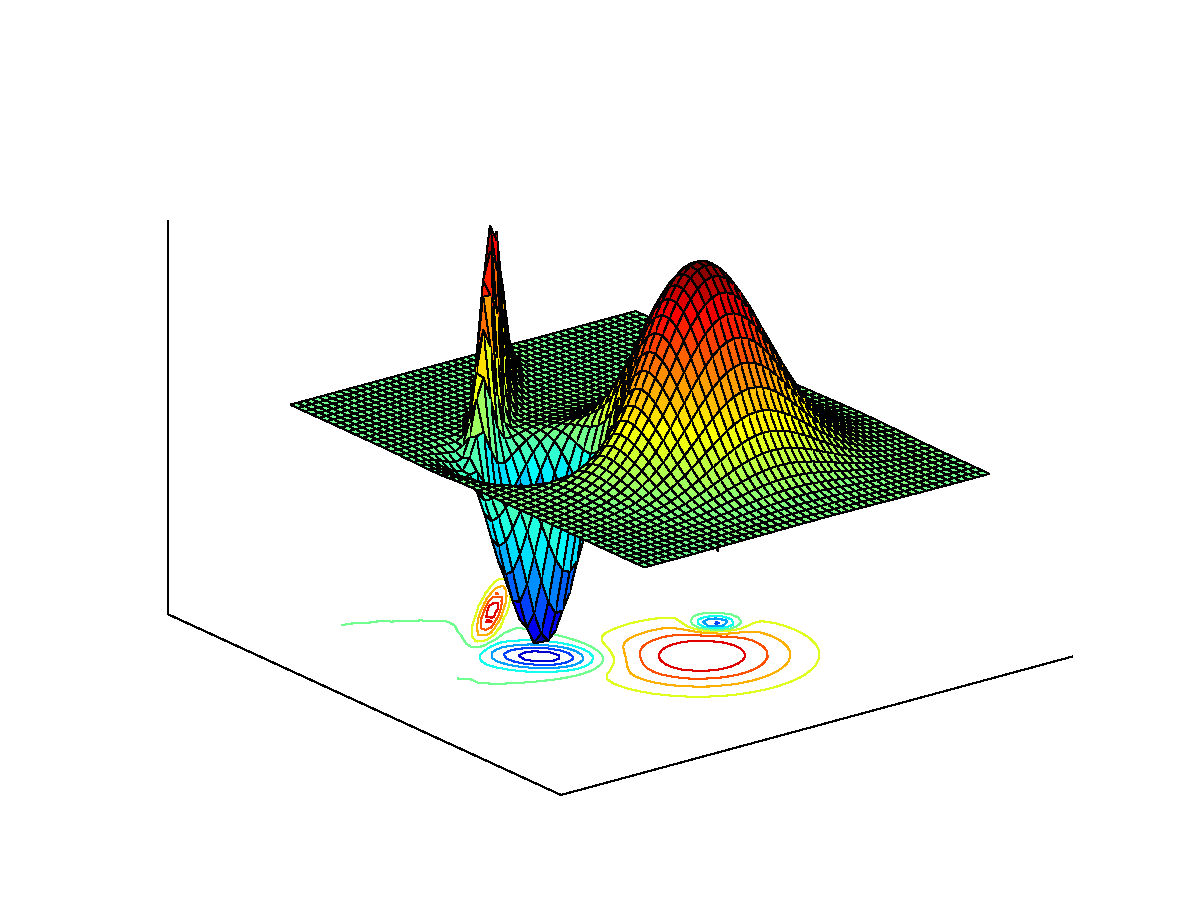
\includegraphics[width=\textwidth]{figures/surface.eps}
        \end{subfigure}
        ~
         \begin{subfigure}[b]{0.45\columnwidth}
                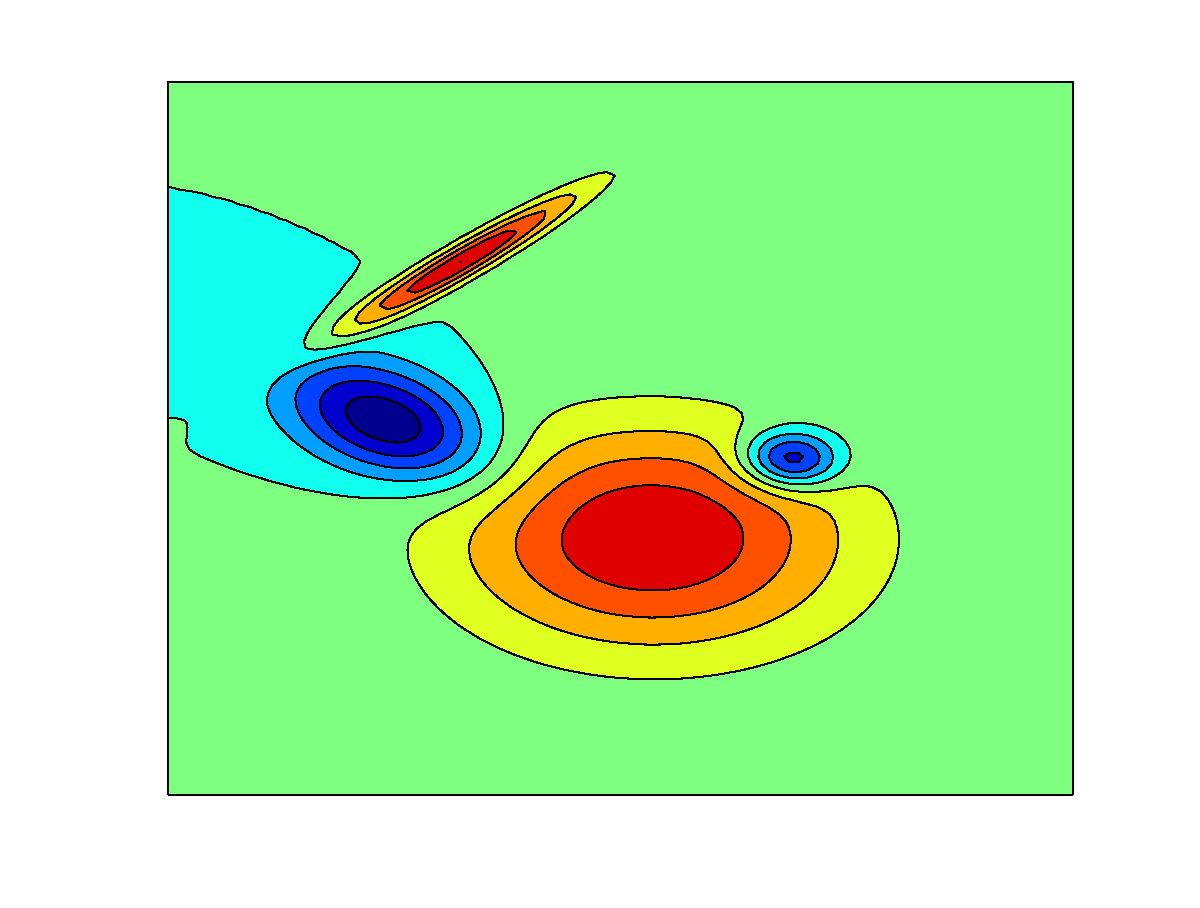
\includegraphics[width=\textwidth]{figures/contour.eps}
        \end{subfigure}
                       
        \caption{Synthetic regression problem generated from a mixture of random Gaussian kernels. }
       \label{fig-toy-example}
\end{figure}
\begin{figure}
        \centering
        \begin{subfigure}[b]{0.3\columnwidth}
               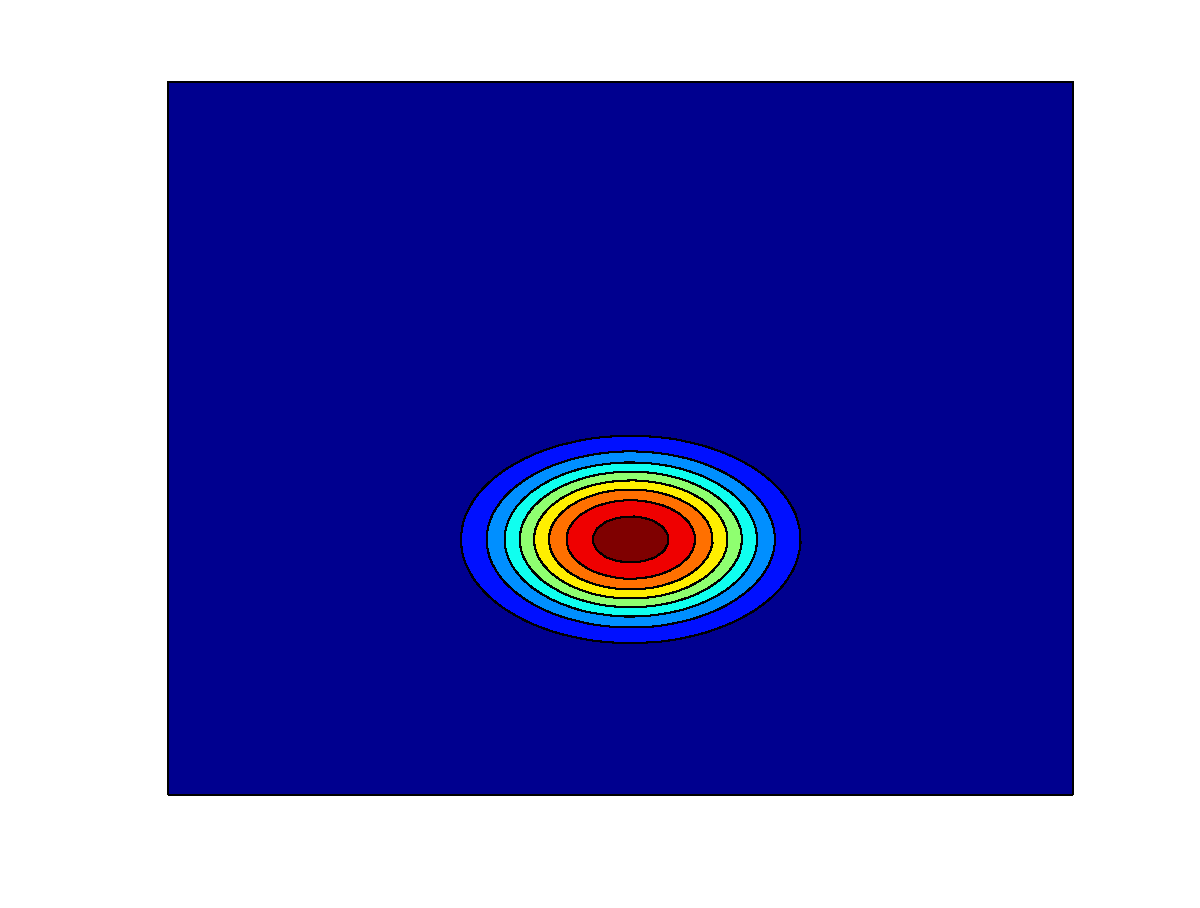
\includegraphics[width=\textwidth]{figures/GPGL1.eps}
        \end{subfigure}
        ~
         \begin{subfigure}[b]{0.3\columnwidth}
                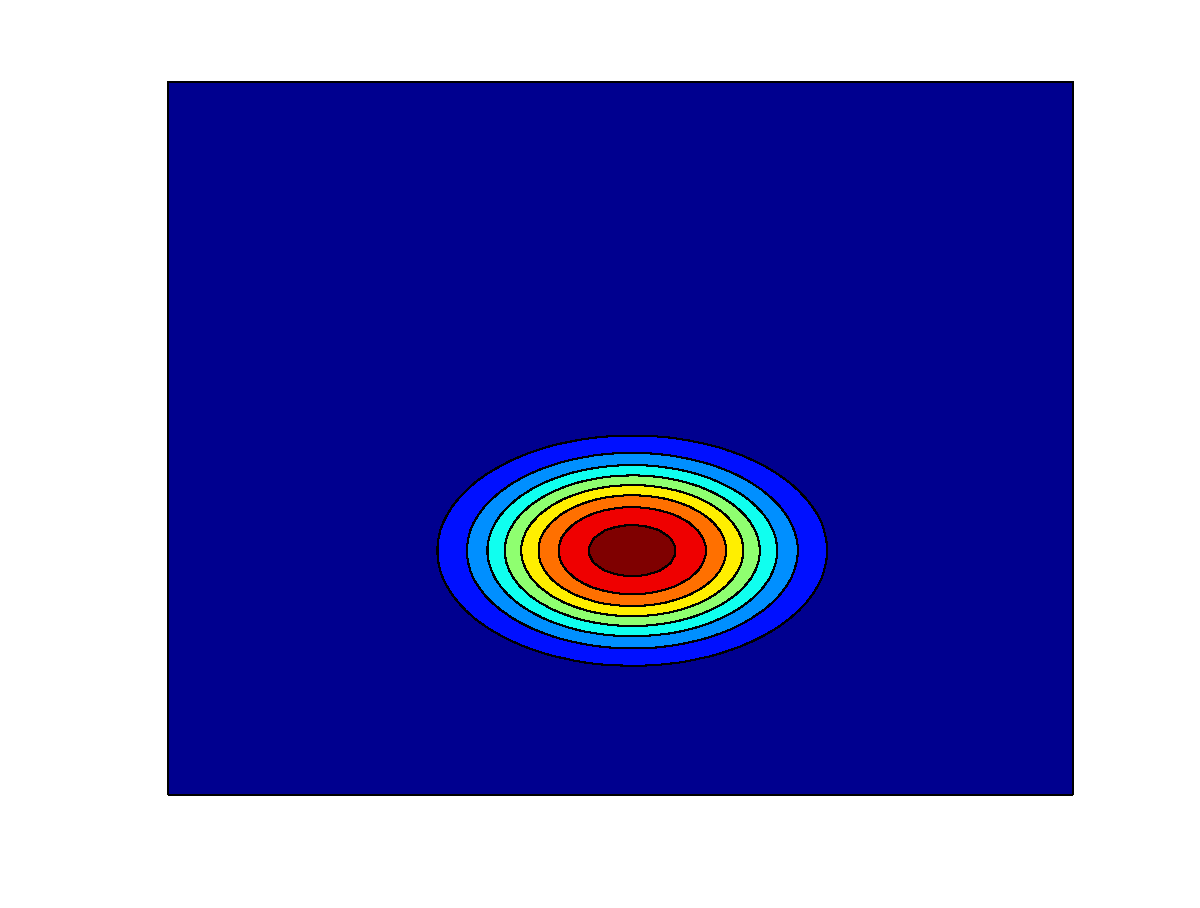
\includegraphics[width=\textwidth]{figures/GPVL1.eps}
        \end{subfigure}
        ~
        \begin{subfigure}[b]{0.3\columnwidth}
               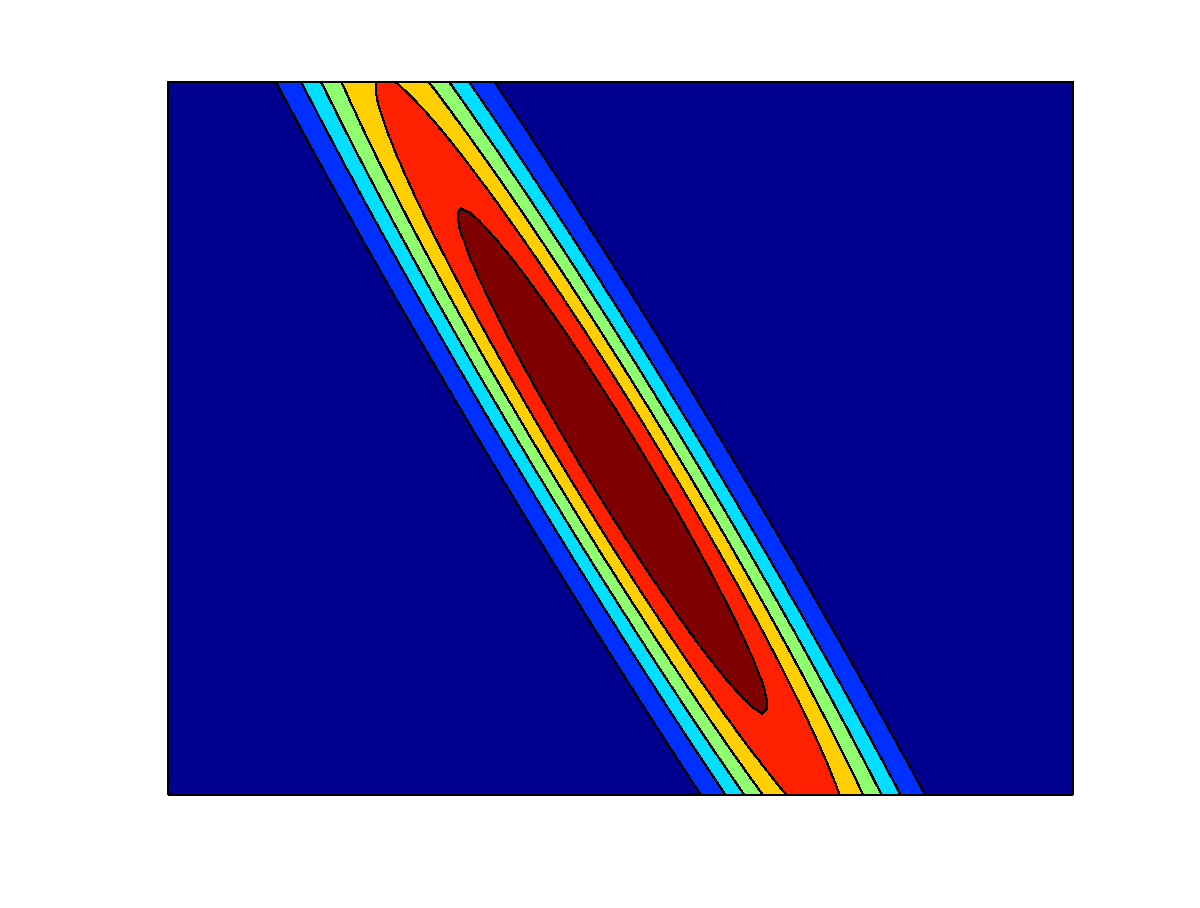
\includegraphics[width=\textwidth]{figures/GPVC1.eps}
        \end{subfigure}
       
         \begin{subfigure}[b]{0.3\columnwidth}
               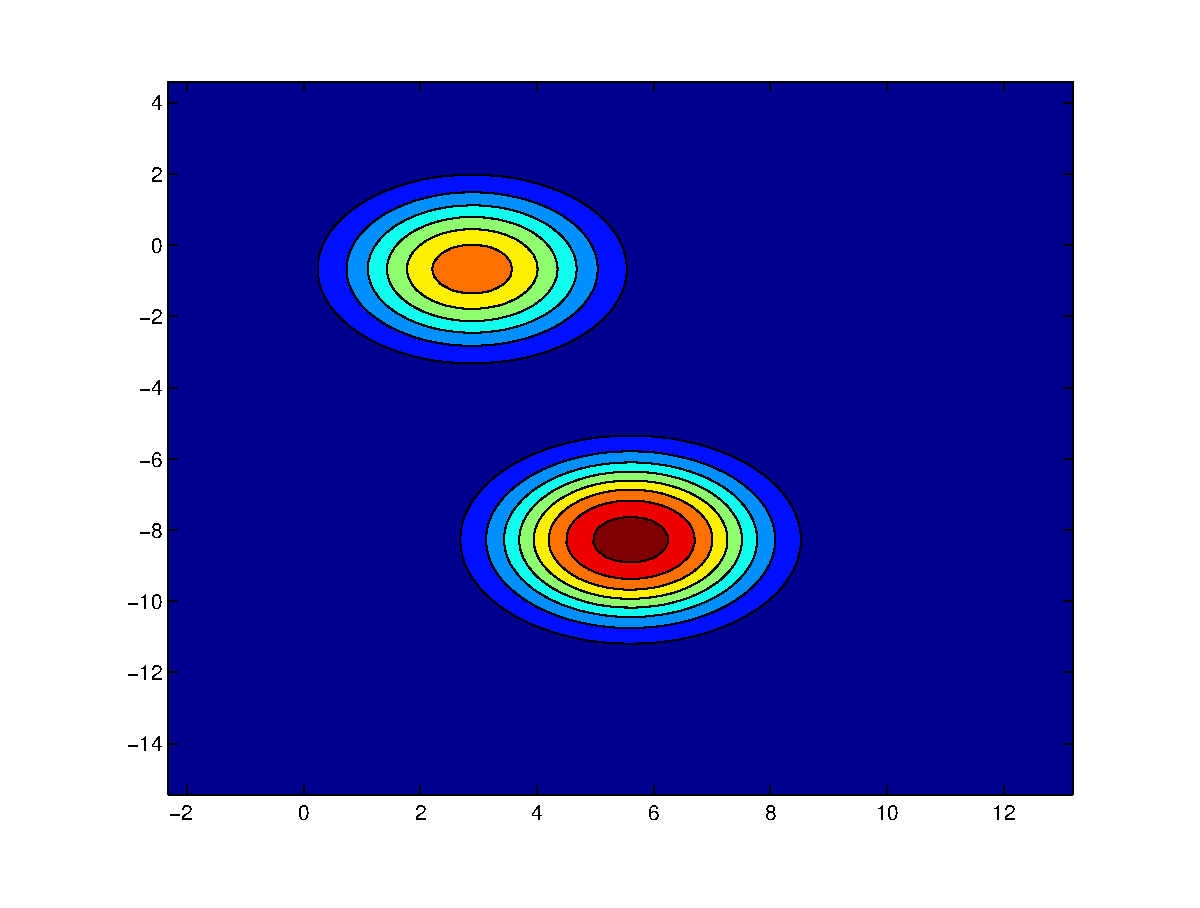
\includegraphics[width=\textwidth]{figures/GPGL2.eps}
        \end{subfigure}
        ~
         \begin{subfigure}[b]{0.3\columnwidth}
               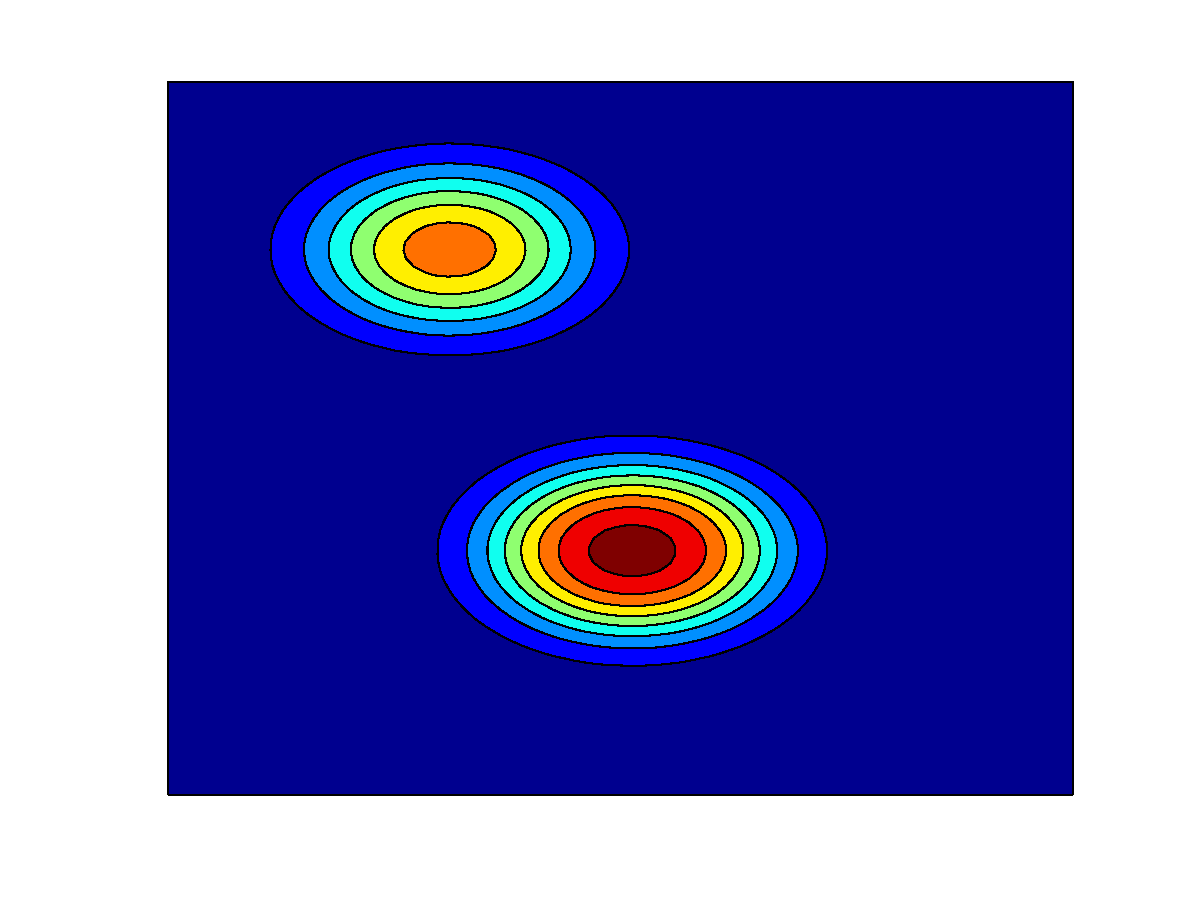
\includegraphics[width=\textwidth]{figures/GPVL2.eps}
        \end{subfigure}
        ~
        \begin{subfigure}[b]{0.3\columnwidth}
                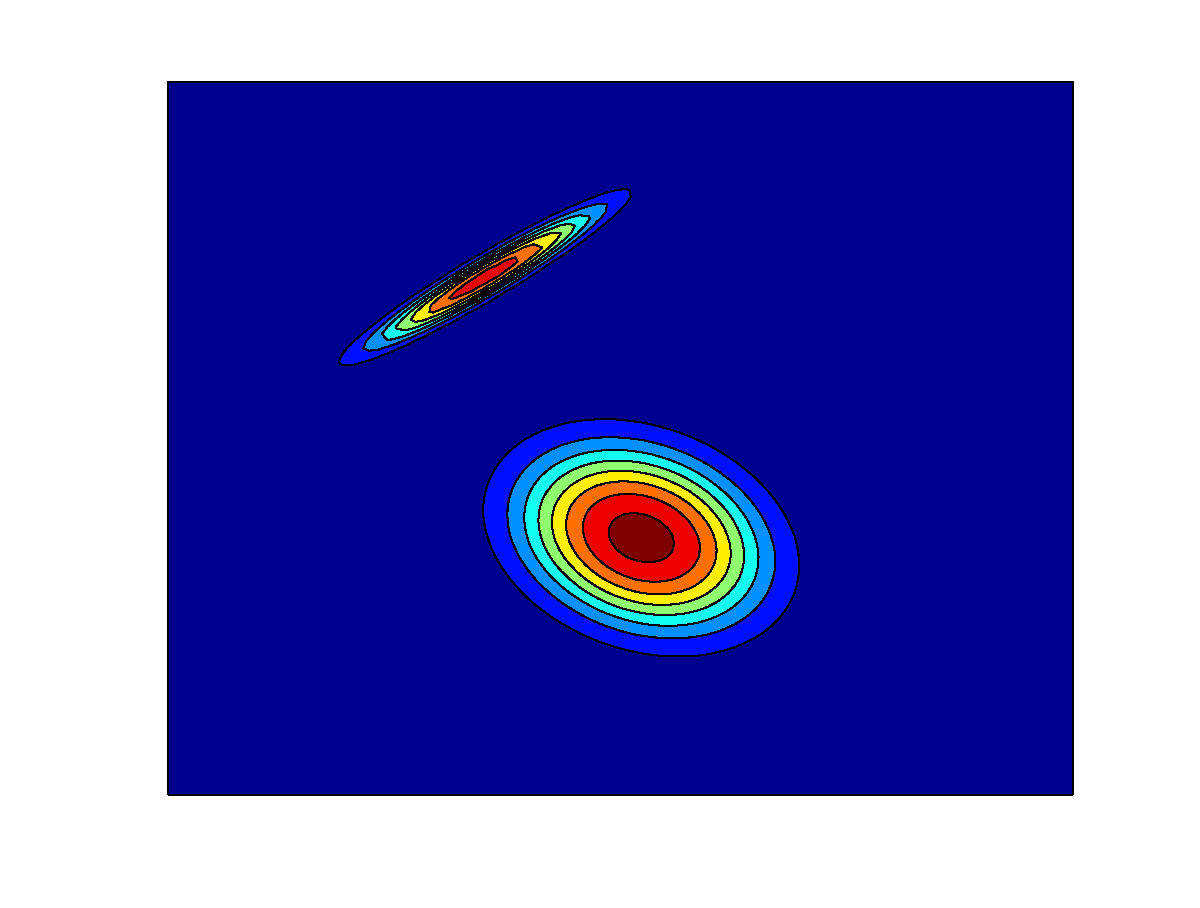
\includegraphics[width=\textwidth]{figures/GPVC2.eps}
        \end{subfigure}
       
         \begin{subfigure}[b]{0.3\columnwidth}
                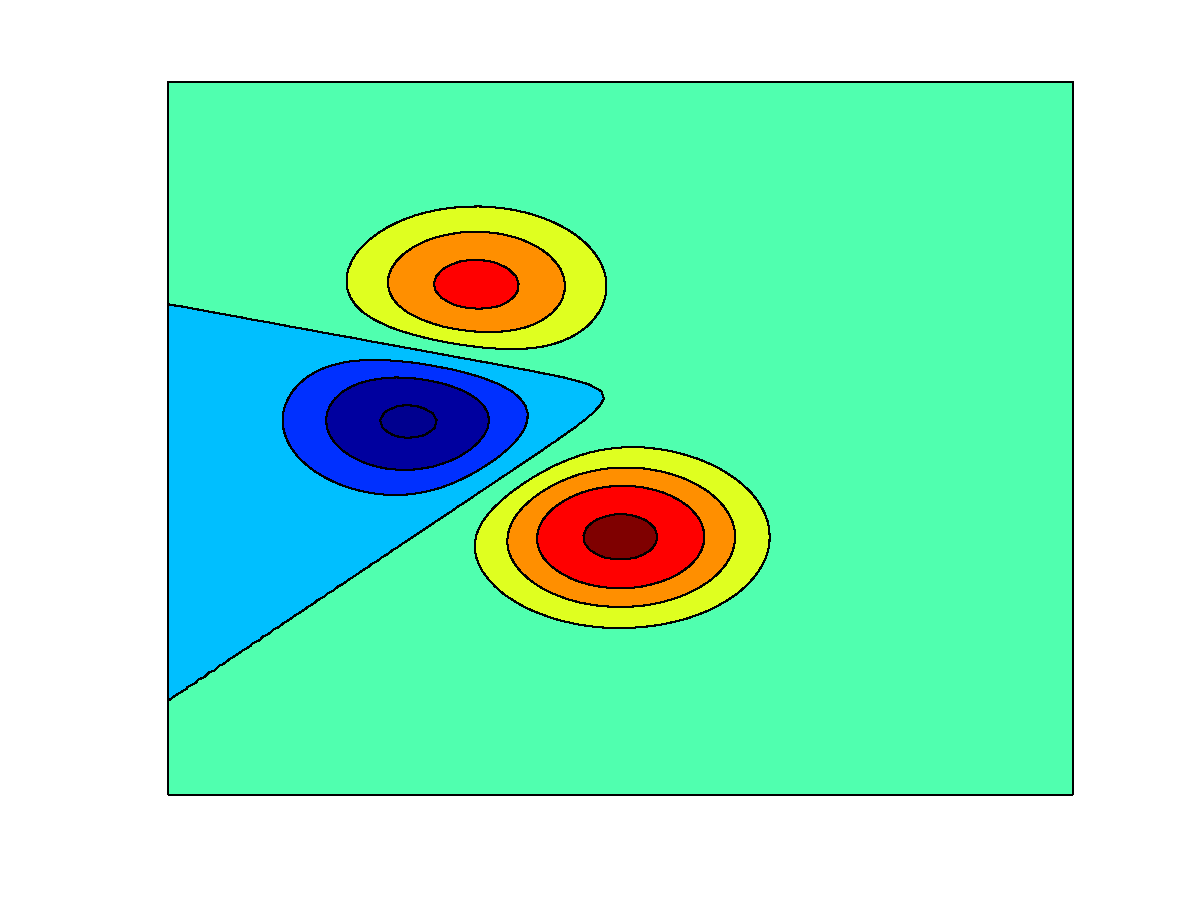
\includegraphics[width=\textwidth]{figures/GPGL3.eps}
        \end{subfigure}
        ~
         \begin{subfigure}[b]{0.3\columnwidth}
                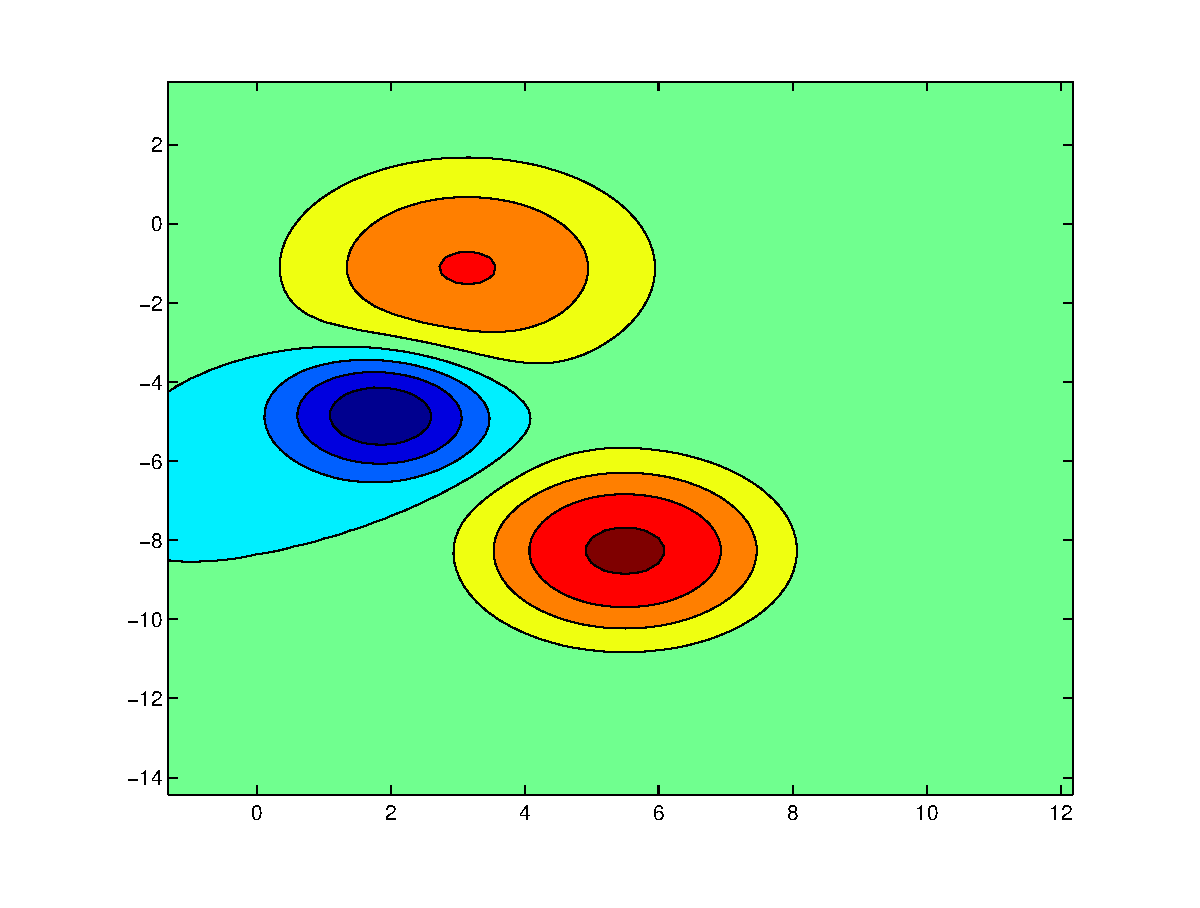
\includegraphics[width=\textwidth]{figures/GPVL3.eps}
        \end{subfigure}
        ~
        \begin{subfigure}[b]{0.3\columnwidth}
                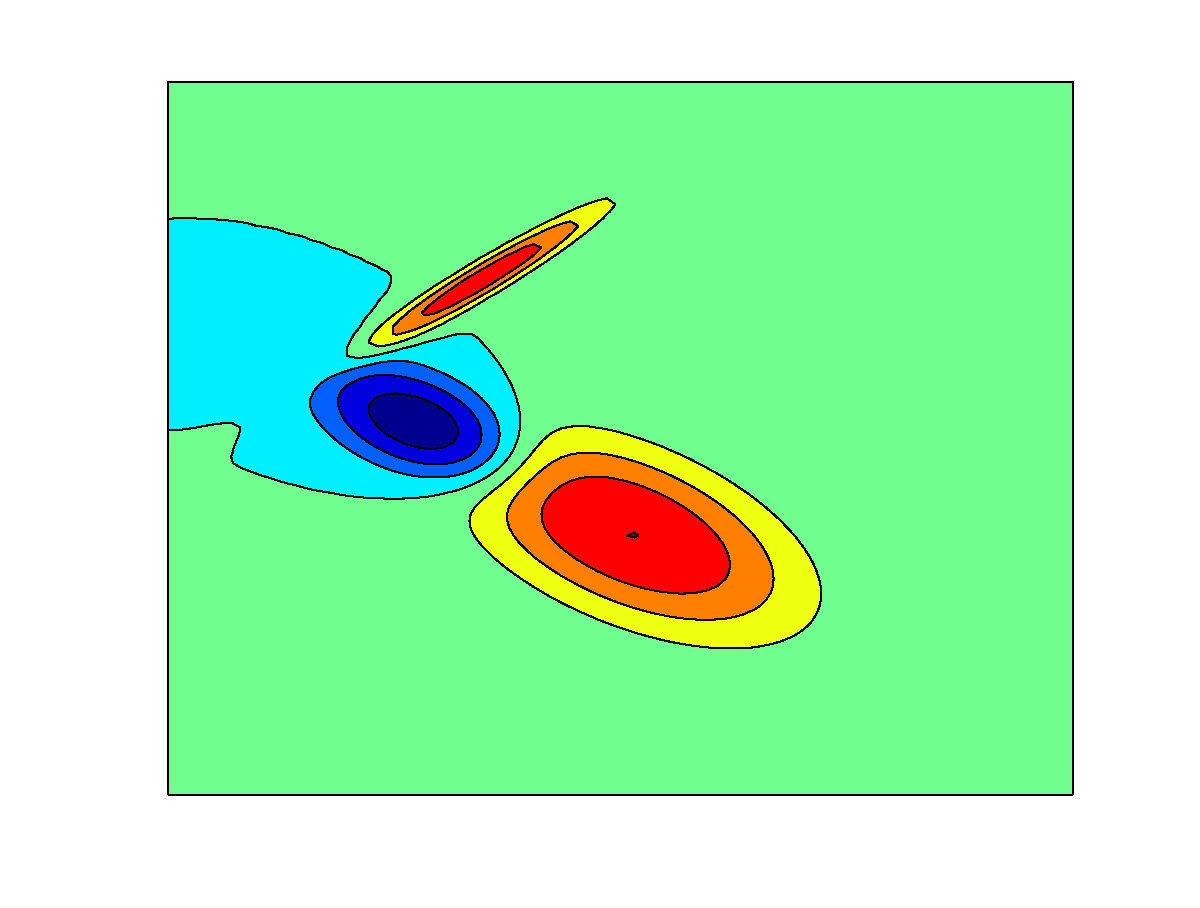
\includegraphics[width=\textwidth]{figures/GPVC3.eps}
        \end{subfigure}
         \begin{subfigure}[b]{0.3\columnwidth}
                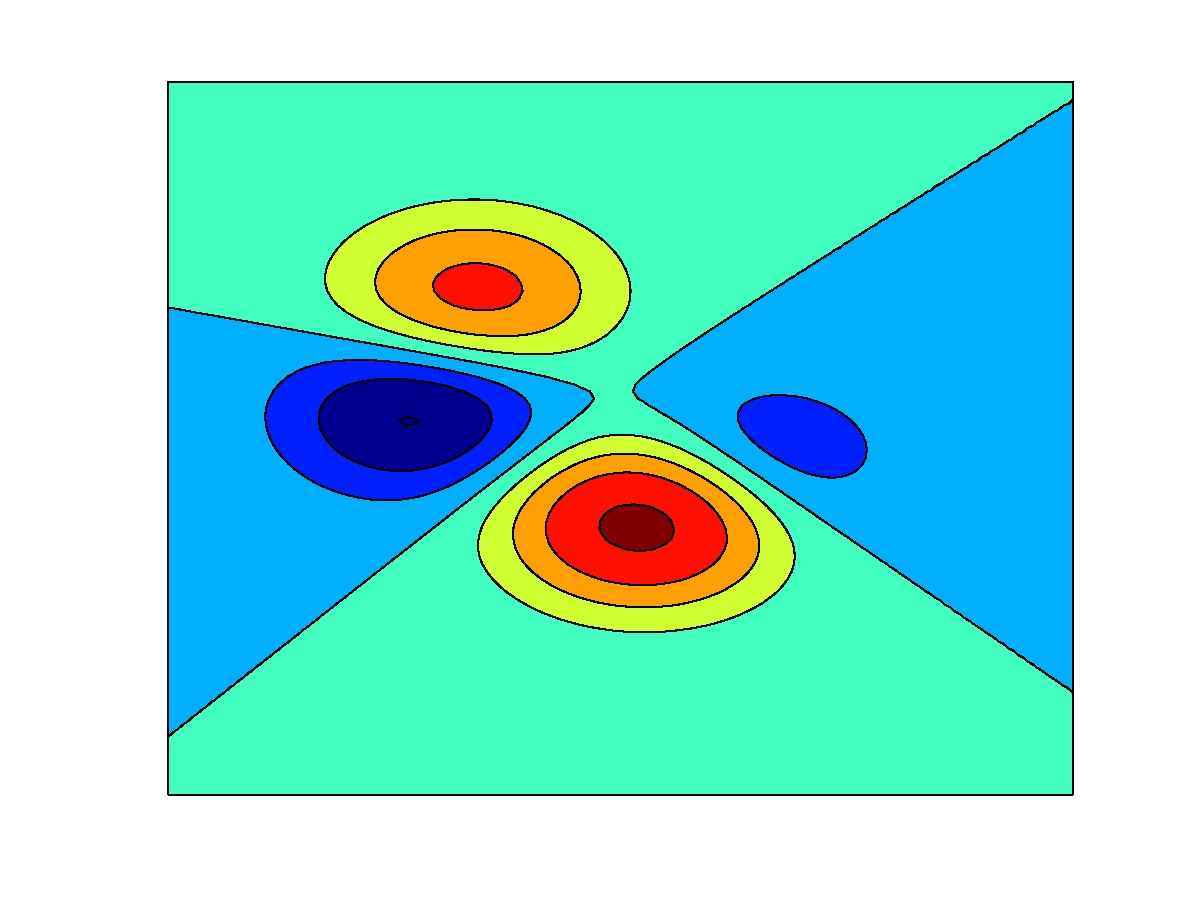
\includegraphics[width=\textwidth]{figures/GPGL4.eps}
                \caption{GP-GL}
        \end{subfigure}
        ~
         \begin{subfigure}[b]{0.3\columnwidth}
                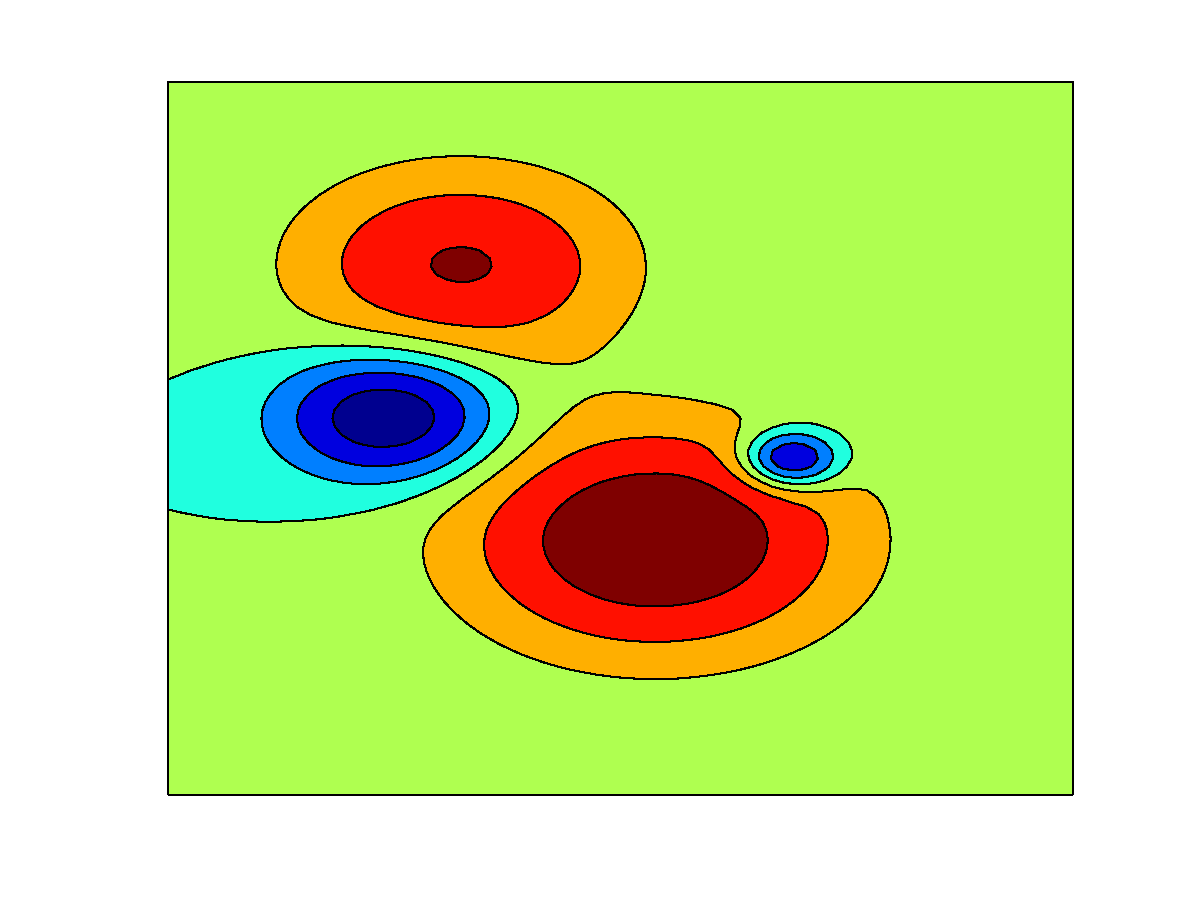
\includegraphics[width=\textwidth]{figures/GPVL4.eps}
                \caption{GP-VL}
        \end{subfigure}
        ~
        \begin{subfigure}[b]{0.3\columnwidth}
                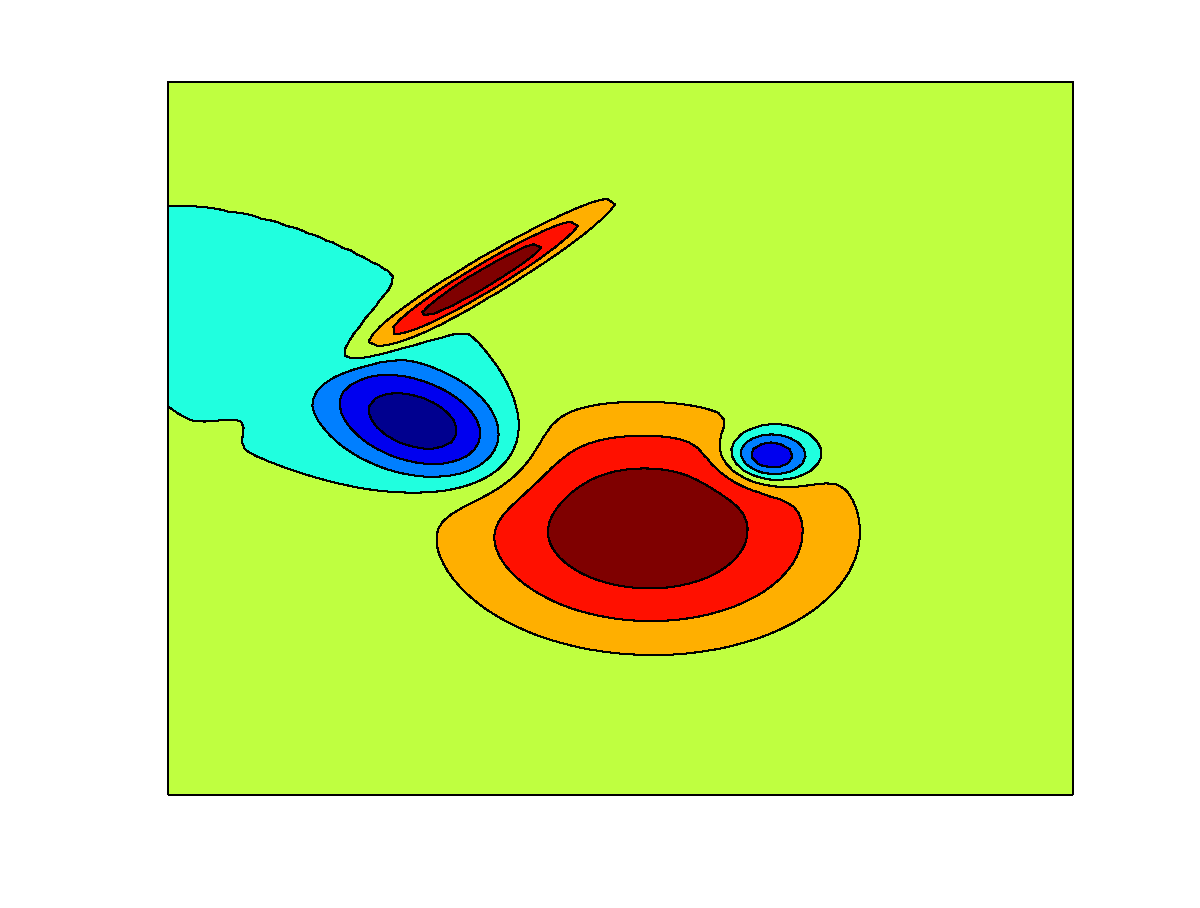
\includegraphics[width=\textwidth]{figures/GPVC4.eps}
                \caption{GP-VC}
        \end{subfigure}          
        \caption{Comparisons between different sparse GP approaches with 1 to 4 basis functions (top to bottom) using (a) a global length scale, (b) variable length scales and (c) variable covariances.}
        \label{fig-toy-comparison}
\end{figure}
\subsection{Linear Regression Prior}

In the absence of observations, all Bayesian models, Gaussian processes included, rely on their priors to provide function estimation. For the case of Gaussian processes this requires us to consider the prior over the function, especially the prior mean. For example, we may consider a mean function that is itself a simple linear regression from the independent to dependent variable. The parameters of this function are thence inferred and the GP infers non-linear deviations. In the absence of data, e.g. in extrapolative regions, the GP will fall back to the linear regression prediction \citep{roberts2012rs}. We can incorporate this directly into the optimisation objective instead of having it as a separate preprocessing step by redefining $\bmath{K}$ as a concatenation of the linear and non-linear features, or setting $\bmath{K}=[\bmath{K}|\bmath{X}|\underset{n}{1}]$. Furthermore, the regularisation matrix in Eq. \eqref{eq-linear-regression-objective-rectangular} can be modified so that it penalises for learning high coefficients for the non-linear terms but no or little cost for learning linear terms by setting the corresponding elements in the diagonal of $I$ to 0, or the last $d+1$ elements. Therefore, as $\sigma_{n}^{2}$ goes to infinity, the model will get closer to a simple linear regression model.

\subsection{Cost Sensitive Learning}

Thus far in the discussion, we make the tacit assumption that the objective of the inference process is to minimise the sum of squared errors between the model and target function values. Although this is a suitable objective for many applications, it is intrinsically biased by uneven distributions of training data in input and output, sacrificing accuracy in less represented regions of the space. Ideally we would like to train a model with distribution balanced data to avoid such bias. This, however, is a luxury that we often do not have. A common technique is to either over-sample or under-sample the data to achieve balance \citep{weiss2007}. In under-sampling, samples are removed from highly represented regions to achieve balance, over-sampling on the other hand duplicates under represented samples. Both approaches come with a cost; in the former good data is wasted and in the latter more computation is introduced due to the data size increase. In this paper, we perform cost-sensitive learning, which increases the intrinsic error function in under-represented regions. In regression tasks, such as we consider here, the output can be either discretised and treated as classes for the purpose of cost assignment, or a probability function is fitted to the output then samples are weighted in proportion to their inverse probability. After the weights have been assigned, they can be incorporated directly into the objective via:
\begin{equation}
\label{eq-weighted-linear-regression-objective}
\begin{array}{lcl}
\underset{w}{\text{min}} &\frac{1}{2}\left ( \bmath{K}w-y \right )^{T} \bmath{W}\left( \bmath{K}w-y \right )+\frac{1}{2}\sigma_{n}^{2}w^{T}w.
\end{array}
\end{equation}

The difference between the objectives in Eq. \eqref{eq-linear-regression-objective} and Eq. \eqref{eq-weighted-linear-regression-objective} is the introduction of the diagonal matrix $\bmath{W}$, where each element $\bmath{W}_{ii}$ is the corresponding cost for sample $i$. The first term in Eq. \eqref{eq-weighted-linear-regression-objective} is a matrix form for a weighted sum of squares $\sum_{i=1}^{n}\bmath{W}_{ii}\left(\bmath{K}_{i,*}w-y_{i}\right)^{2}$, where the solution can be found analytically as follows:
\begin{equation}
\label{eq-weighted-linear-regression-objective-rectangular}
w = \left(\bmath{K}^{T}\bmath{WK}+\bmath{I}\sigma_{n}^{2} \right)^{-1}\bmath{K}^{T}\bmath{W}y.
\end{equation}
The only modification to the gradient calculation is to set the matrix $\bmath{E}=\bmath{W}\left(\left(\bmath{K}w-y\right)w^{T}\right)\circ\bmath{K}$.

\section{Application to Photometric Redshift Estimation}
\label{sec-application}

%Here we consider the problem of redshift estimation from photometric data. The aim of this approach is to predict accurately the redshift from the magnitudes of different colour bands emitted by a source using photometry. The light for each band is filtered to measure the magnitude of a particular wavelength range. 


Here, we specifically target the photometric configuration designed for the Euclid Space Mission. The Euclid telescope provides near-infrared data in a broad RIZ band and the more standard Y, J and H bands, while ground-based ancillary data are expected in the optical g, r, i and z bands. 


\subsection{Dataset}
\label{sec-dataset}

The dataset is a mock catalogue from \citet{jouvel09}, consisting of the g, r, i, z, RIZ, Y, J and H magnitudes (to 10$\sigma$ depths of 24.6, 24.2, 24.4, 23.8, 25.0 for the former, and 5$\sigma$ depth of 24.0 for each of the latter three) for 156,904 simulated sources along with their spectroscopic redshift. We restrict ourselves to the redshift range of $0.2 \le z_{spec} \le 2$ to target the requirements set by the Euclid Space Mission in this specific range. All sources with any missing measurement in any of their detectors were removed prior to training. No additional limits on any of the bands were used, although some will be explicitly removed to test the extrapolation performance of the models. The distribution of the spectroscopic redshift is provided in Figure \ref{fig-zspec-hostogram}. For all experiments reported in this paper, we ignore the error bars associated with each band and train only on the magnitudes. In all experiments reported in this paper, the data is preprocessed using Principle Component Analysis (PCA) \citep{jolliffe1986} to de-correlate the features prior to learning. De-correlation accelerates the convergence rate of the optimisation routine especially when using a logistic-type kernel machines such as Neural Networks \citep{lecun1998}. To understand this, we consider a simple linear regression example where we would like to solve for $w$ in $Aw=b$, the solution for this is $w=\left(A^{T}A\right)^{-1}A^{T}b$. Note that if $A$ is de-correlated $A^{T}A=I$, therefore learning $w_{i}$ depends only on the $i$-th column of $A$ and it is independent from learning $w_{j}$, where $i\ne j$. In an optimisation approach, the convergence rate is a function of the condition number of the $A^{T}A$ matrix, which is minimised in the case of de-correlated data. This represents a quadratic error surface which helps accelerate the search. This is particularly important in the application addressed in this paper as the colour bands are strongly correlated with each other. An example of applying a simple coordinate-descent to optimise a linear regression model was applied to the toy data set and the results are shown in Figure \ref{fig-error-surface}.

\begin{figure}
        \centering
        \begin{subfigure}[b]{0.45\columnwidth}
                 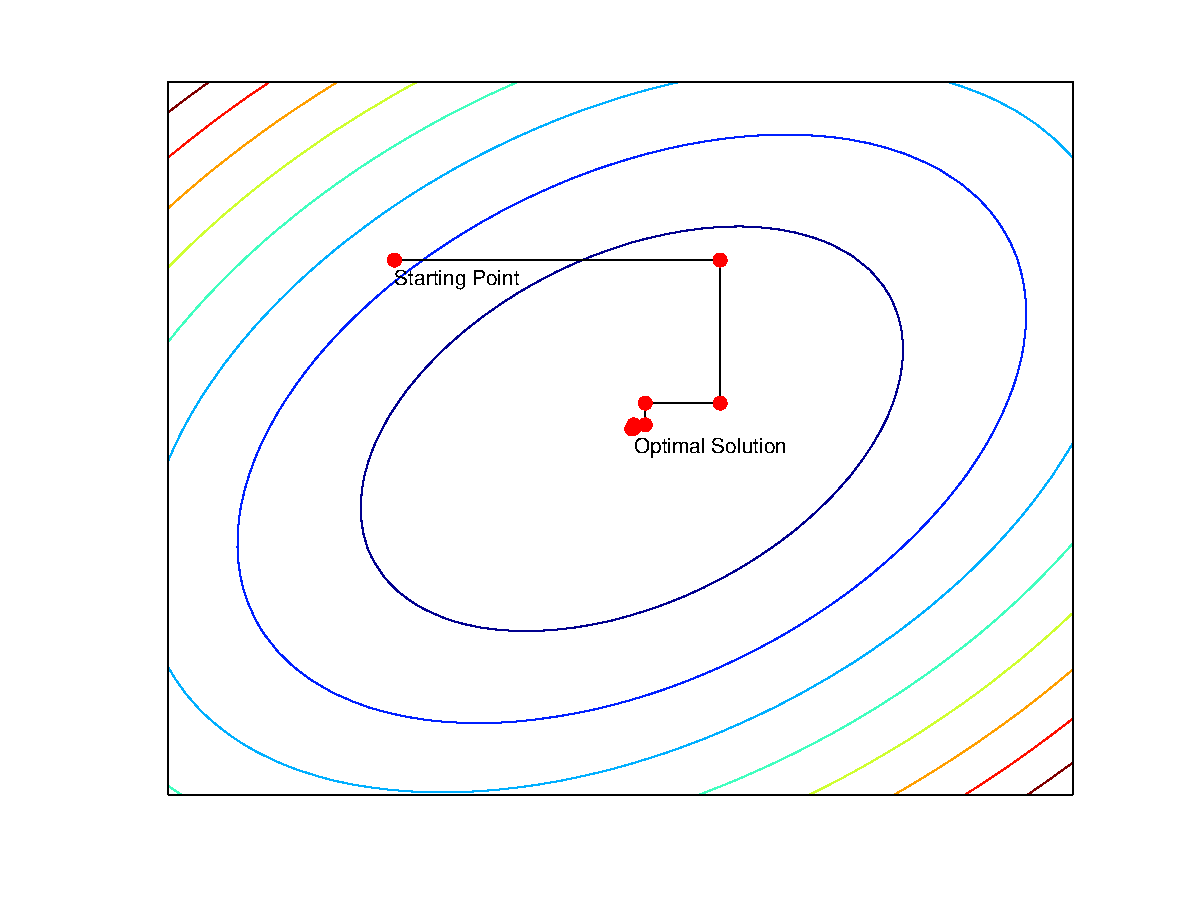
\includegraphics[width=\textwidth]{figures/correlated.eps}
                 \caption{Correlated}
        \end{subfigure}
        ~
        \begin{subfigure}[b]{0.45\columnwidth}
                 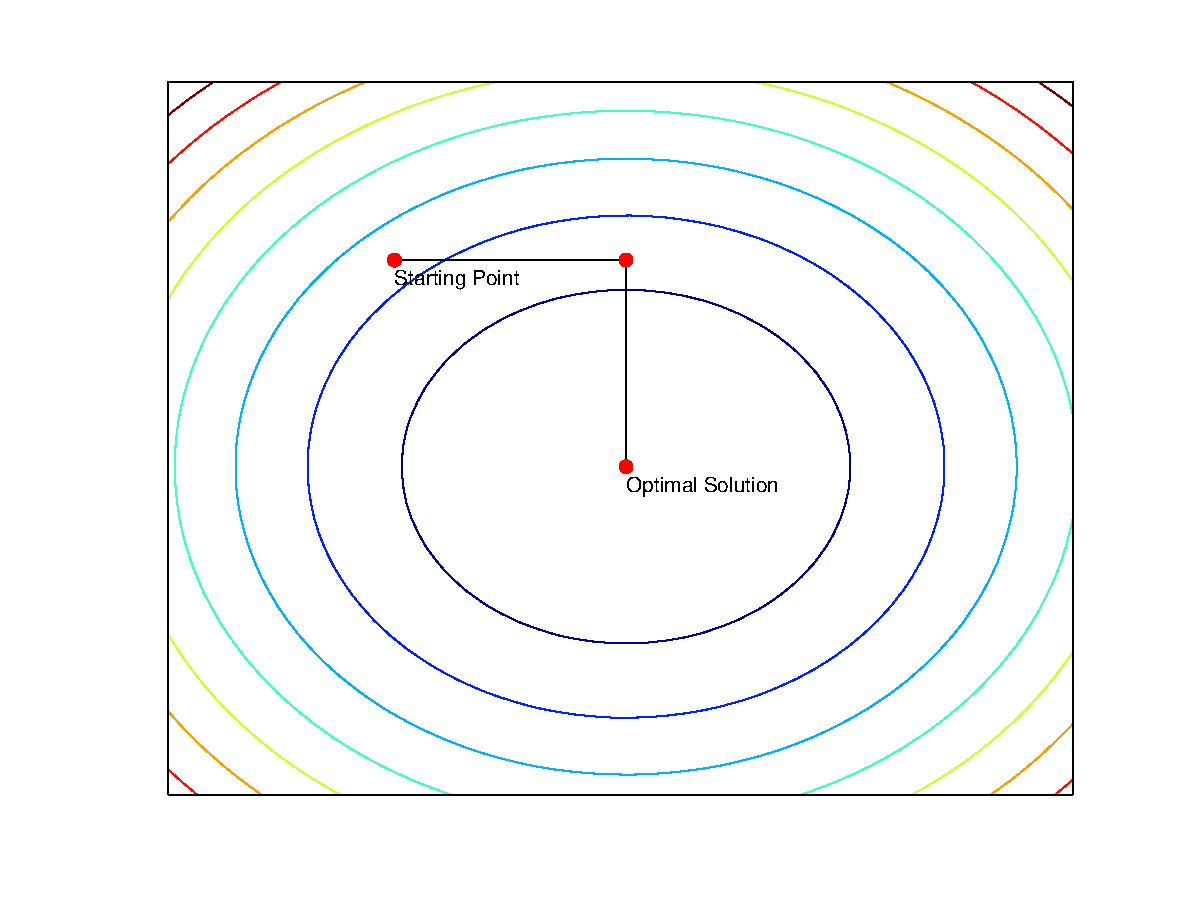
\includegraphics[width=\textwidth]{figures/decorrelated.eps}
                 \caption{De-correlated}
        \end{subfigure}
       \caption{Using coordinate-descent to optimise the linear regression objective on the synthetic dataset shown in Figure \ref{fig-toy-example}. Subfigure (a) shows the steps taken when the data has some correlation, while subfigure (b) shows the steps taken when the data was de-correlated.}
	\label{fig-error-surface}
\end{figure}
\begin{figure}
       \centering
       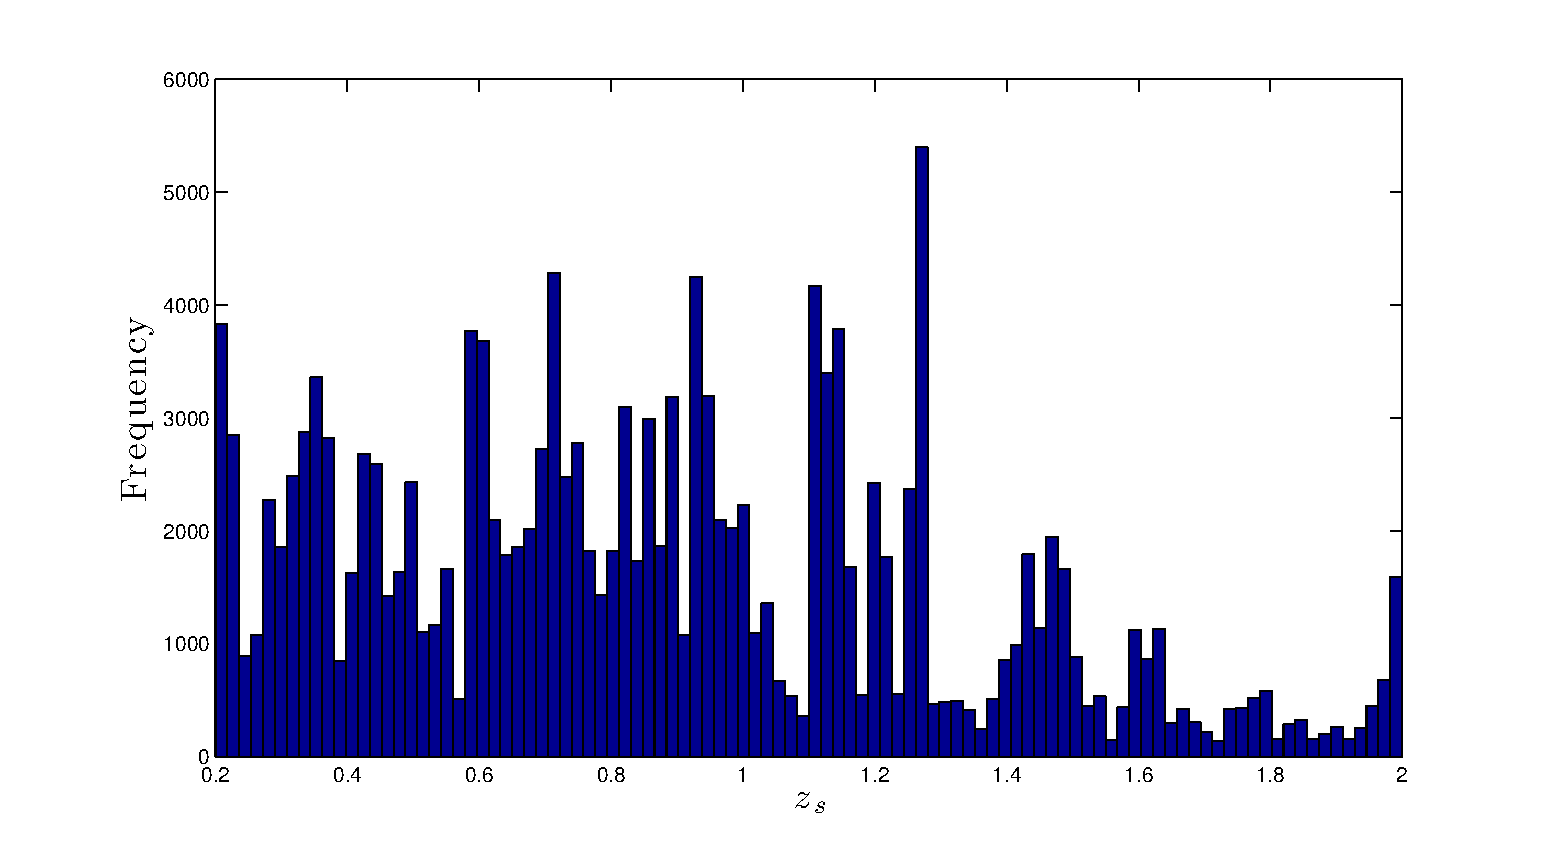
\includegraphics[width=\columnwidth]{figures/zspec.eps}
        \caption{The spectroscopic redshift distribution of the full dataset.}
       \label{fig-zspec-hostogram}
\end{figure}

\section{Experiments and Results}
\label{sec-experiments}

Five algorithms are considered to model the data; Artificial Neural Networks (ANN), a GP with low rank approximation (stableGP), a sparse GP with global length scale (GP-GL), a GP with variable length scale (GP-VL) and a GP with variable covariances (GP-VC). For the ANN, a single layer network is used with hyperbolic tangent hidden activations and linear output activations, for the low rank approximation GP we use the SR-VP method proposed in \citep{foster2009}. In subsequent tests, the variable $m$ refers to the number of hidden units in ANN, the rank in stableGP, and the number of basis functions in GP-GL, GP-VL and GP-VC. The data was split at random into 80\% for training, 10\% for validation and 10\% for testing. The validation set was used for model selection and all the results here are reported on the test set. The following performance measures on the test set are reported for each experiment:
\begin{itemize}
  \item $\Delta z_{\phantom{norm}} = \sqrt{\frac{1}{n}\sum_{i=1}^{n}\left(z_{spec}-z_{phot}\right)^{2}}$
  \item $\Delta z_{norm} = \sqrt{\frac{1}{n}\sum_{i=1}^{n}\left(\frac{z_{spec}-z_{phot}}{1+z_{spec}}\right)^{2}}$,
\end{itemize}
in which $\Delta z$ is the standard Root Mean Squared Error (RMSE) and $\Delta z_{norm}$ is a normalised version that weights low redshift objects more aggressively than higher redshift objects. The scientific goal of the Euclid mission is to reach a $\Delta z_{norm} \le 0.05$ \citep{laureijs2011}.

\subsection{Modelling Performance}

In the first test, all models were trained using a fixed $m=10$ to cross compare the performance of the methods using the same number of basis functions. The number of basis functions was set deliberately low to highlight the sparse-limit modelling capabilities of each algorithm, as for large values of $m$ the performance gap between the algorithms naturally becomes less. The standard sum of squares objective was used, without cost sensitive training or a prior mean function to keep the comparison as simple as possible. The $z_{spec}$ vs $z_{phot}$ density scatter plots are shown in Figure \ref{fig-experiment-1} and their performance scores are reported in Table \ref{table-experiment-1}.
\begin{figure*}
        \centering
        \begin{subfigure}[b]{0.3\textwidth}
                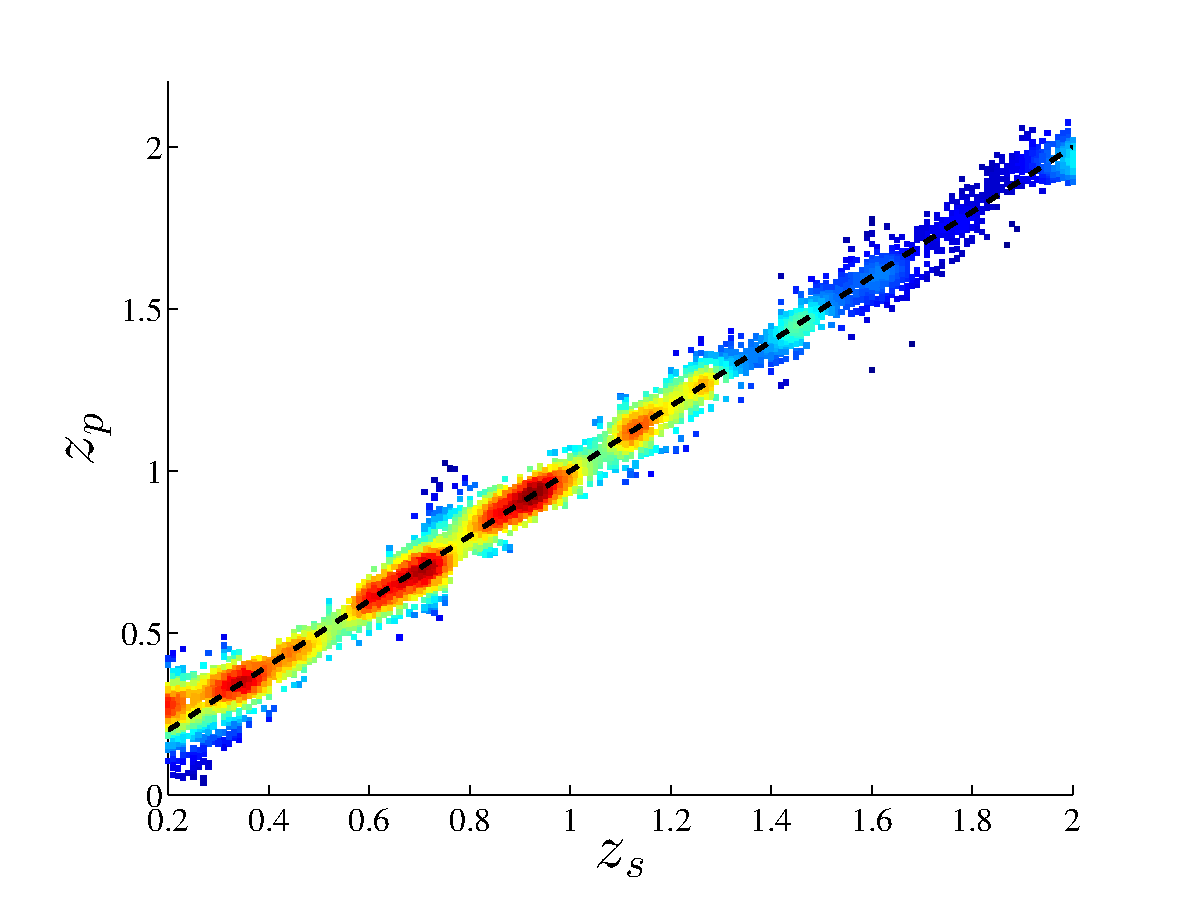
\includegraphics[width=\textwidth]{figures/ANN.eps}
                \caption{ANN}
        \end{subfigure}
        ~
        \begin{subfigure}[b]{0.3\textwidth}
                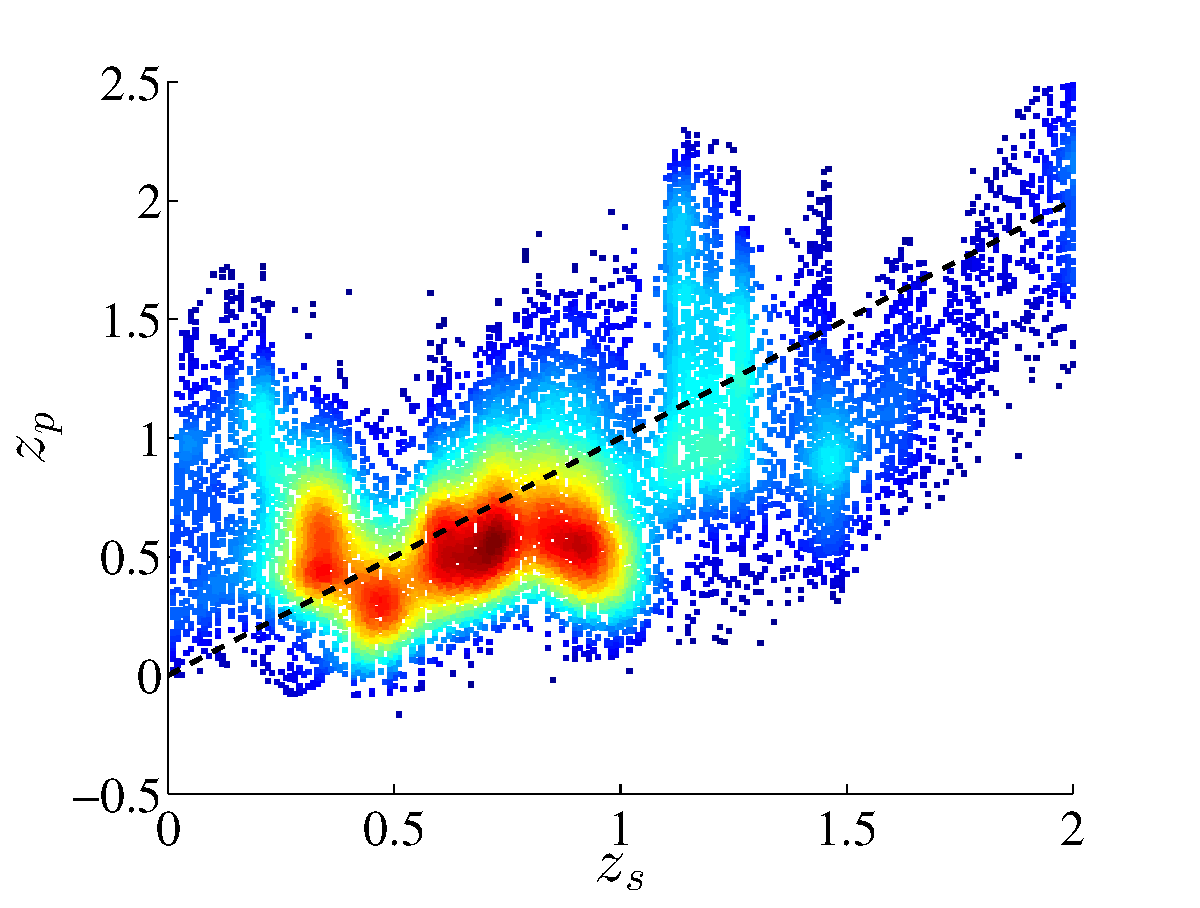
\includegraphics[width=\textwidth]{figures/stableGP.eps}
                \caption{stableGP}
        \end{subfigure}
        ~
        \begin{subfigure}[b]{0.3\textwidth}
                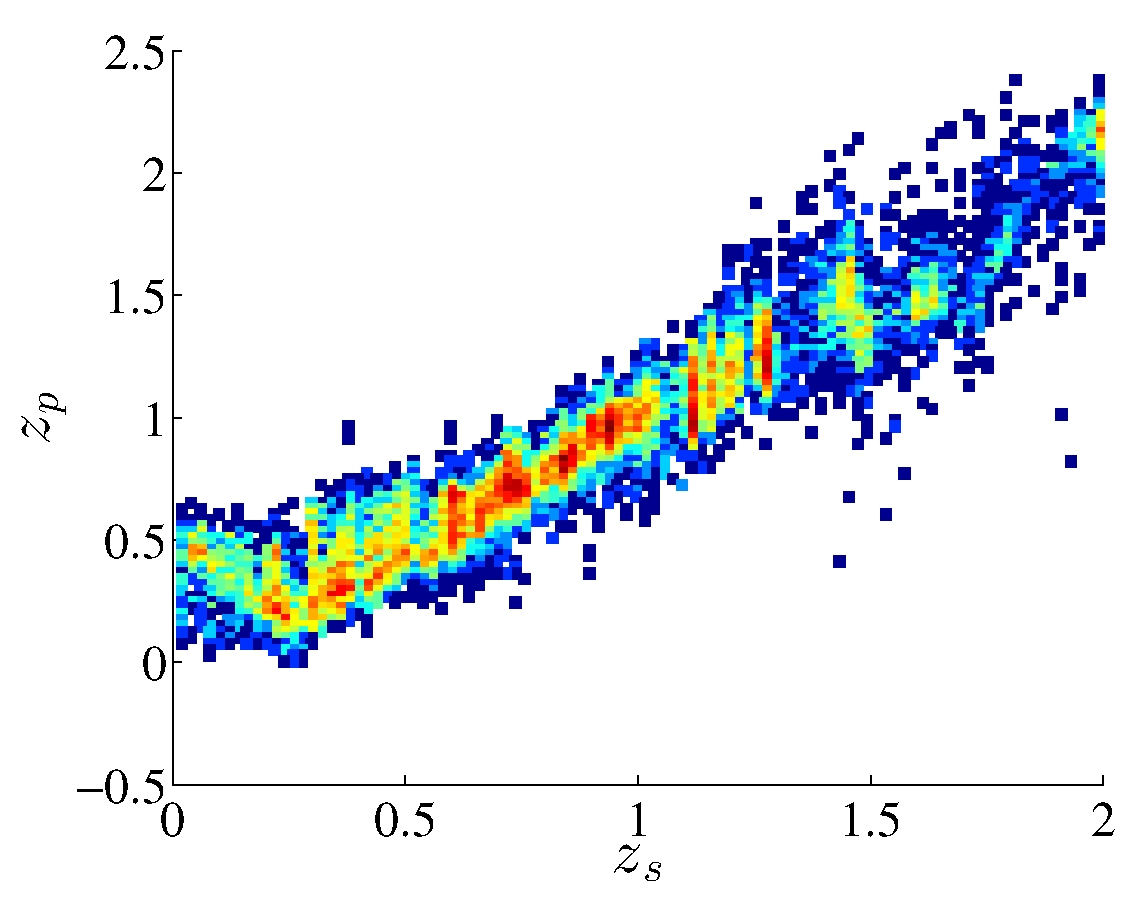
\includegraphics[width=\textwidth]{figures/GPGL.eps}
                \caption{GP-GL}
        \end{subfigure}
        
        \begin{subfigure}[b]{0.3\textwidth}
               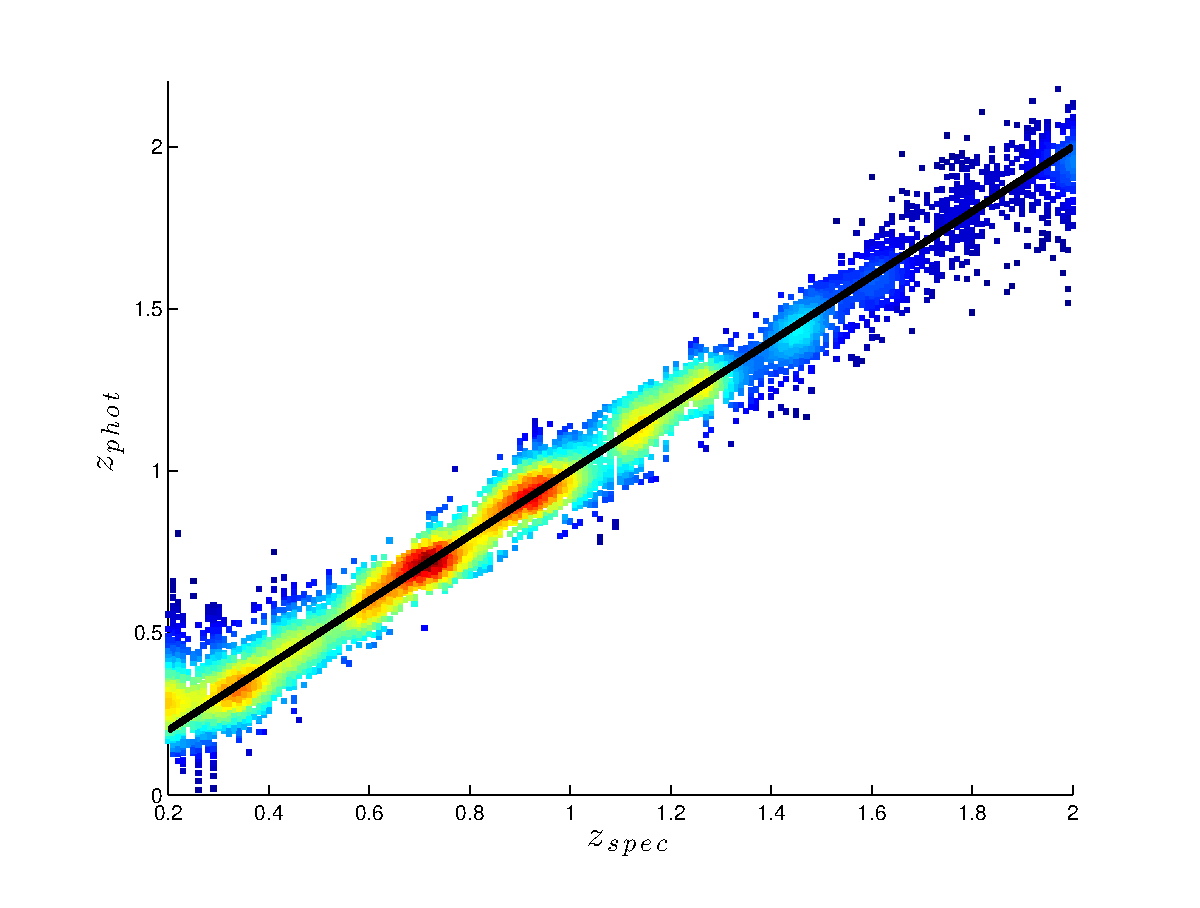
\includegraphics[width=\textwidth]{figures/GPVL.eps}
                \caption{GP-VL}
        \end{subfigure}
        ~
        \begin{subfigure}[b]{0.3\textwidth}
                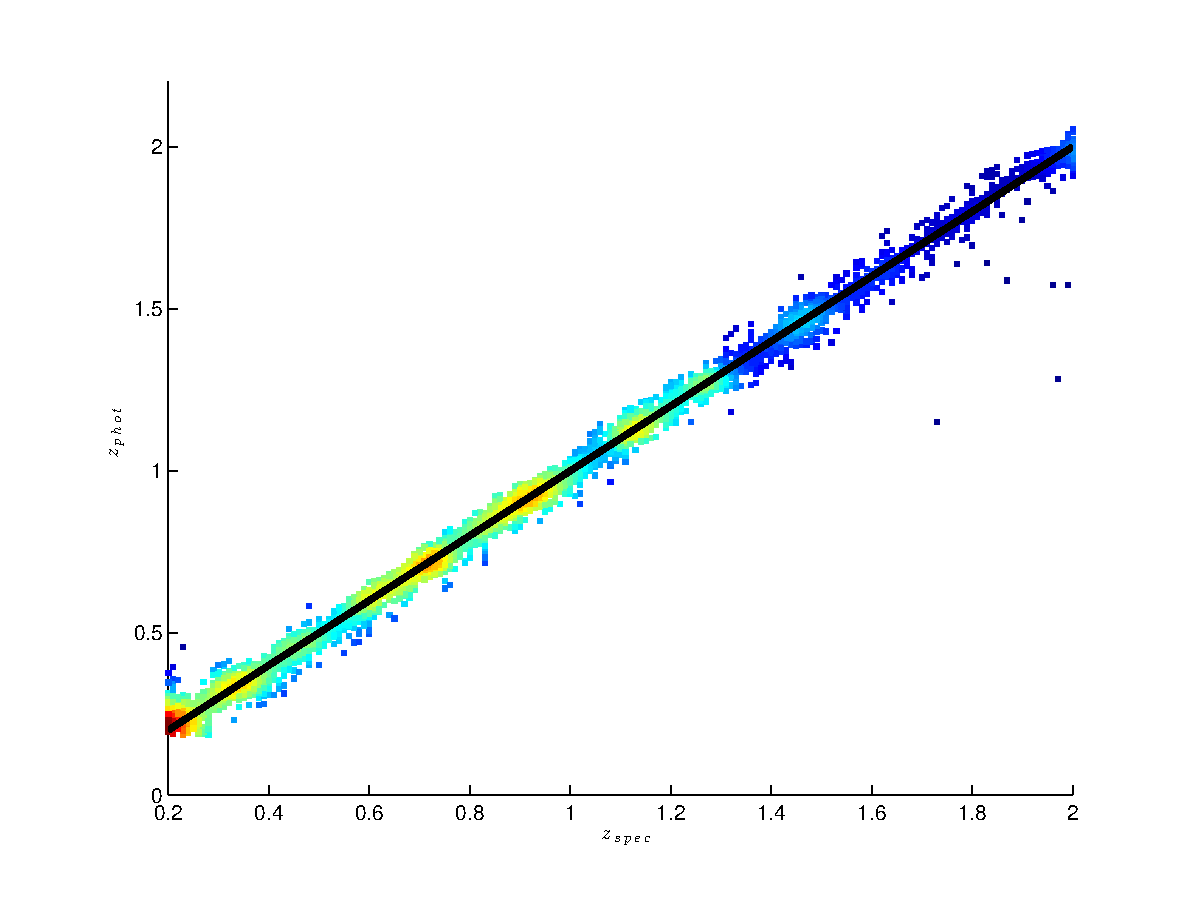
\includegraphics[width=\textwidth]{figures/GPVC.eps}
                \caption{GP-VC}
        \end{subfigure}
        
        \caption{Density scatter plots of the true $z_{spec}$ vs the predicted $z_{phot}$ for (a) ANN, (b) stableGP, (c) GP-GL, (d) GP-VL and (e) GP-VC using $m=10$ basis functions.}
        \label{fig-experiment-1}
\end{figure*}

 \begin{table}
\caption{Performance measures for each algorithm trained using $m=10$ basis functions.}
\begin{center}
  \begin{tabular}{| l | c | c | }
     				&	$\Delta z$	&	$\Delta z_{norm}$	\\	\hline
	ANN			&	0.0423			&	0.0257				\\
	stableGP		&	0.2708			&	0.1559				\\
	GP-GL		&	0.0656			&	0.0399				\\
	GP-VL		&	0.0635			&	0.0394				\\
	GP-VC		&	\textbf{0.0247}		&	\textbf{0.0148}			\\	\hline
  \end{tabular}
  \label{table-experiment-1}
\end{center}
\end{table}

\subsection{Prior Mean}

In this test, the extrapolation performance of the GP-VC model was tested using different prior means, namely a zero mean, a linear regression mean and a joint optimisation approach which learns the linear and non-linear features simultaneously by regularising the non-linear features more aggressively than linear features. To test this more effectively,  the models were trained using sources, with $RIZ<23$ (26,367 objects from the training set) and tested on the unseen samples with $RIZ\ge23$, $RIZ<23$ and the entire test set. A similar test was also conducted using a split of $RIZ<22$ (10,629 objects  from the training set). This also demonstrates the effectiveness of the algorithms in the anticipated scenario where only the brightest sources will have known spectra and therefore can be used for training. The results are reported in Table \ref{table-RIZ-splits} and the density scatter plots are shown for comparison in Figure \ref{fig-RIZ-splits}. The results from Table \ref{table-RIZ-splits} show that the ``Joint'' method consistently outperformed the other methods in extrapolation as well as in interpolation especially when trained with a small sample size as in the $RIZ<22$ case, and upon examining the density scatter plots in Figure \ref{fig-RIZ-splits}, it has less systematic and catastrophic errors.

 \begin{table*}
\caption{The $\Delta z$ for each algorithm trained using $m=10$ basis functions}
\begin{center}
  \begin{tabular}{| l | c | c | c | c | c | c | c | }
  							& 	\multicolumn{3}{|c|}{Trained on $RIZ<22$}				&	& 	\multicolumn{3}{c}{Trained on $RIZ<23$} \\ \cline{2-4} \cline{6-8} 
     	Tested on					&	$<22$			&	$\ge 22$		&	All				&	&	$<23$	&	$\ge 23$	&	All	\\	\hline
	Zero						&	0.0196			&	0.3462			&	0.3311			&	&	0.0239	&	0.0771	&	0.0693					\\
	Linear Regression			&	0.0158			&	0.2394			&	0.2289			&	&	0.0157	&	0.0502	&	0.0452				\\
	Joint						&	\textbf{0.0129}	&	\textbf{0.1144}	&	\textbf{0.1095}	&	&	\textbf{0.0145}	&	\textbf{0.0385}	&	\textbf{0.0349}			\\	\hline
  \end{tabular}
\end{center}
\label{table-RIZ-splits}
\end{table*}

\begin{figure*}
        \centering
        \begin{subfigure}[b]{0.3\textwidth}
                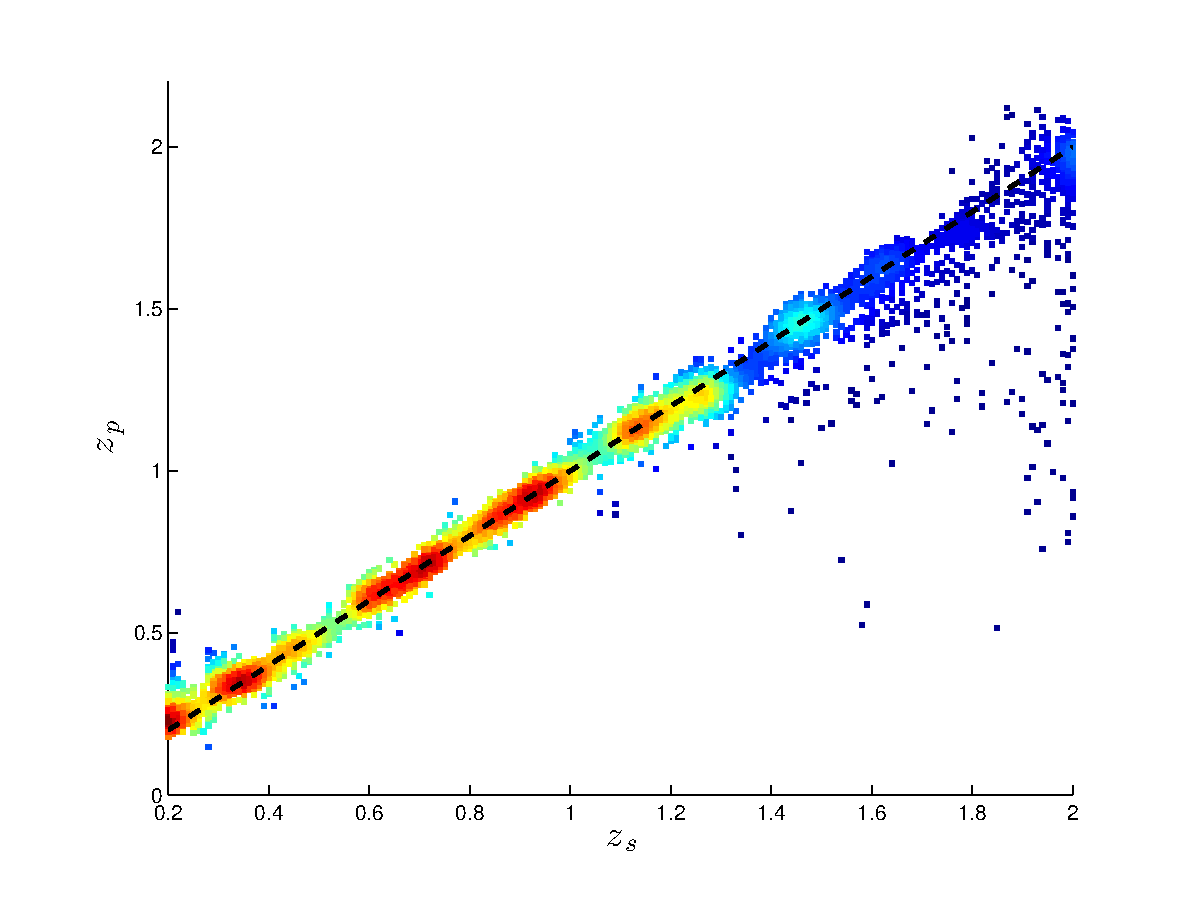
\includegraphics[width=\textwidth]{figures/23_0.eps}
        \end{subfigure}
        ~
        \begin{subfigure}[b]{0.3\textwidth}
                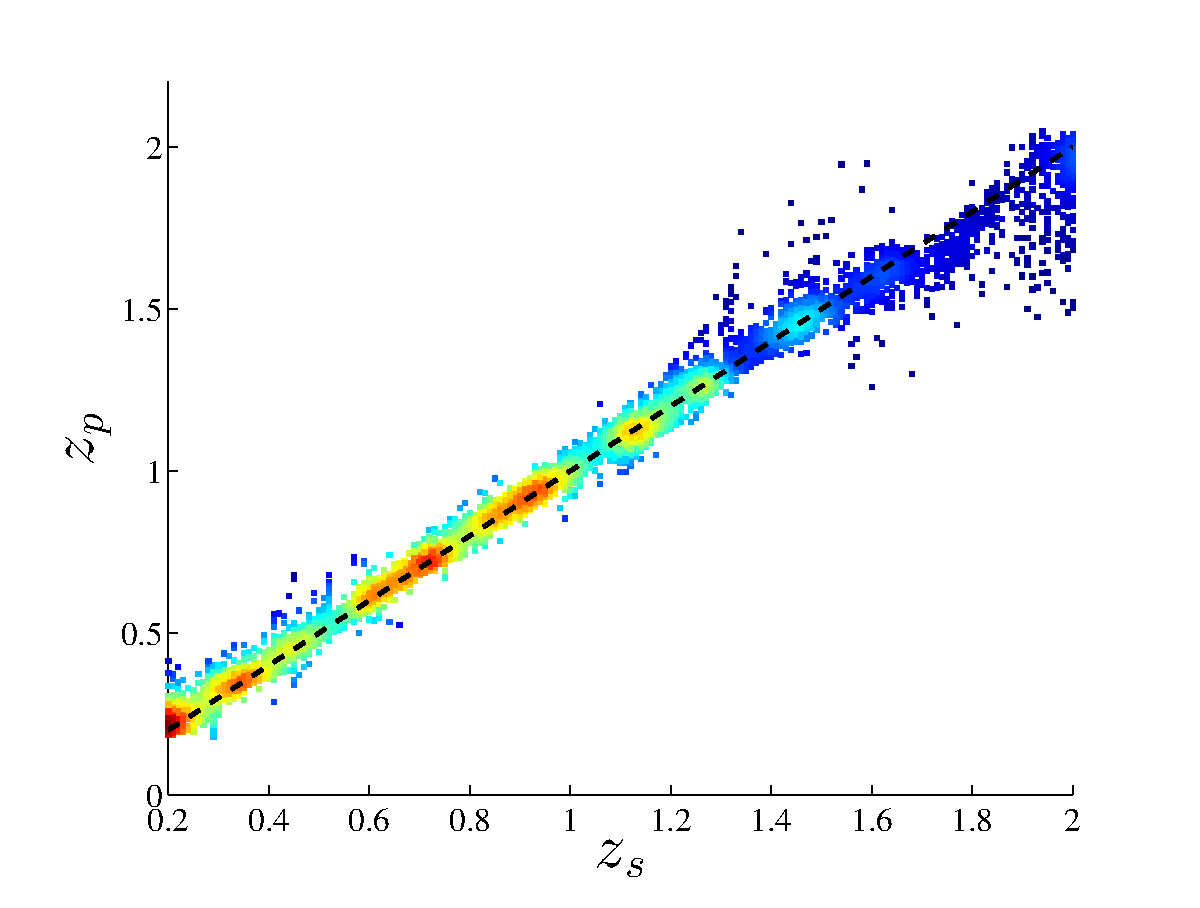
\includegraphics[width=\textwidth]{figures/23_L.eps}
        \end{subfigure}
        ~
        \begin{subfigure}[b]{0.3\textwidth}
                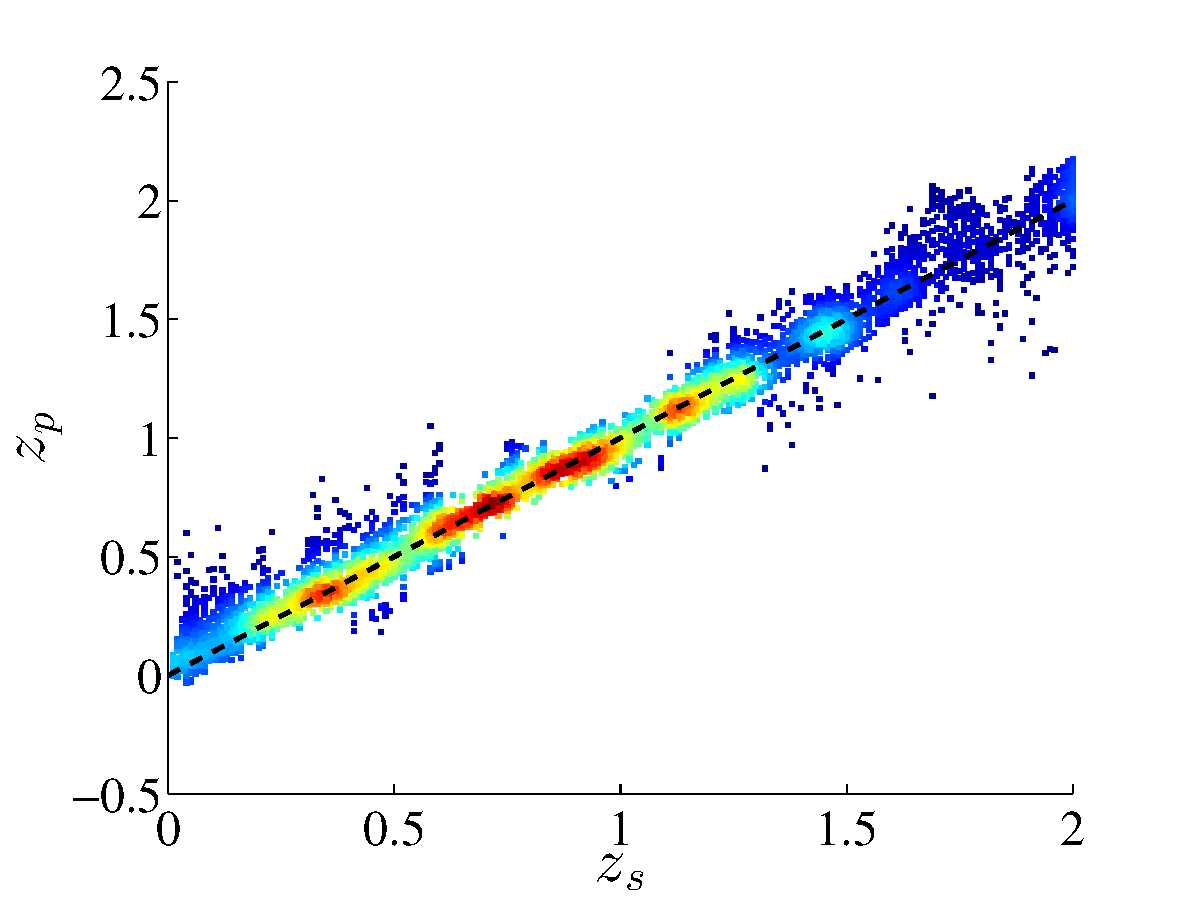
\includegraphics[width=\textwidth]{figures/23_J.eps}
        \end{subfigure}
        
       \begin{subfigure}[b]{0.3\textwidth}
                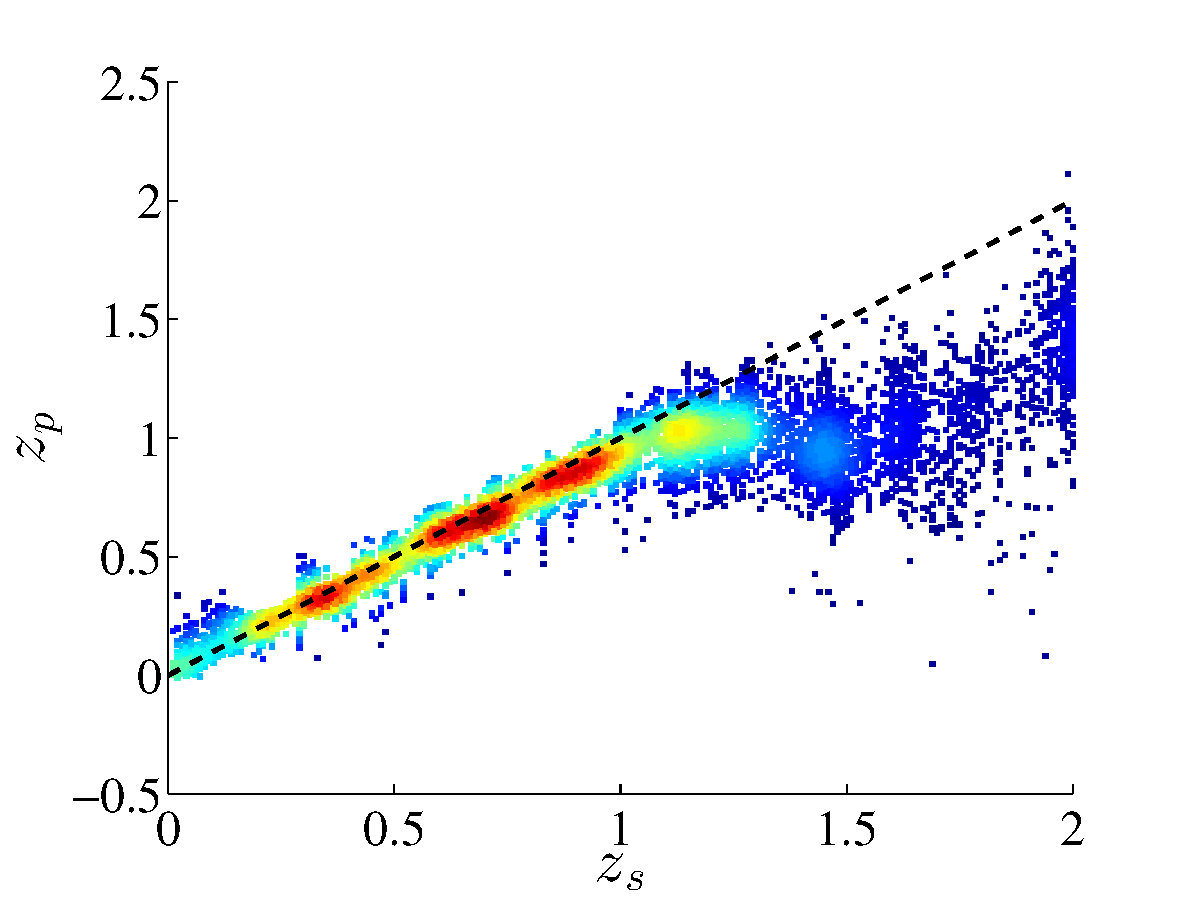
\includegraphics[width=\textwidth]{figures/22_0.eps}
                \caption{Zero mean}
        \end{subfigure}
        ~
        \begin{subfigure}[b]{0.3\textwidth}
                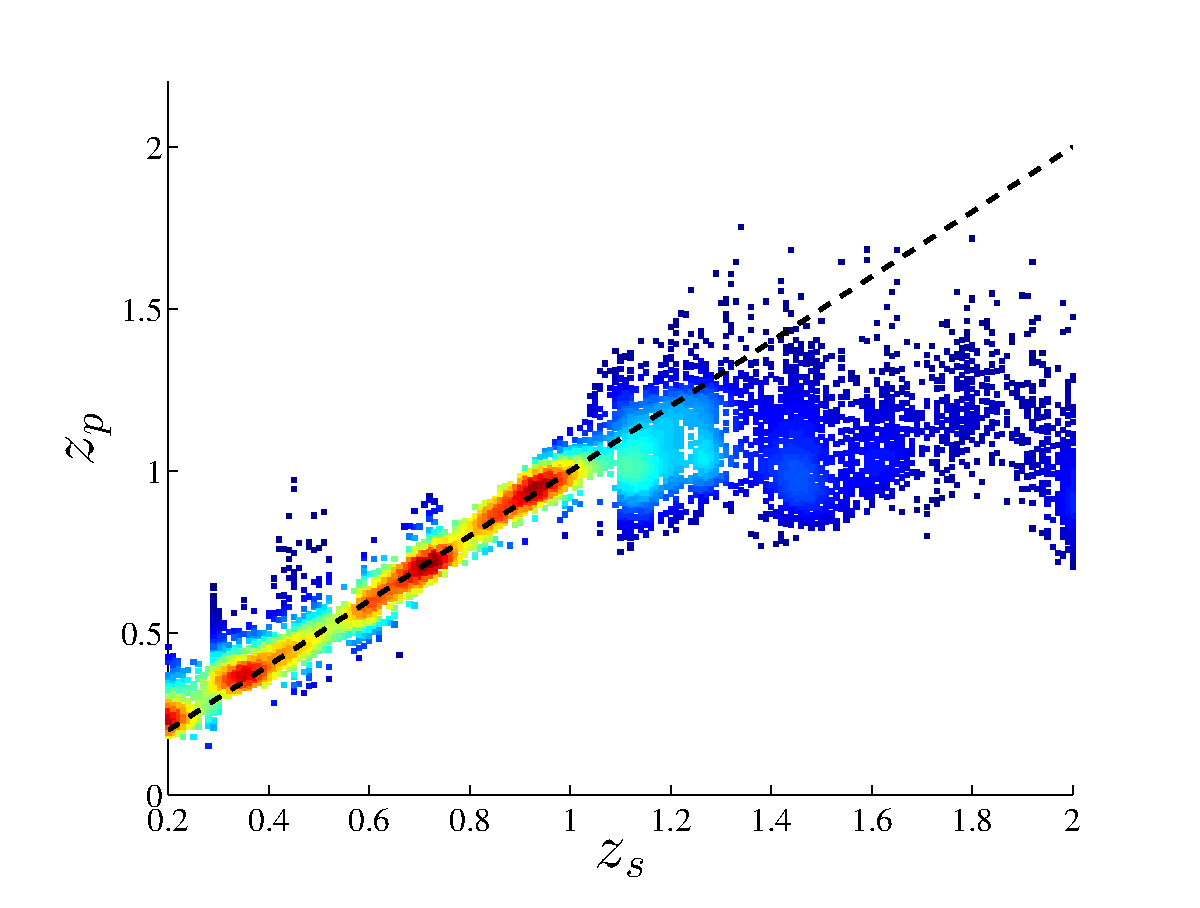
\includegraphics[width=\textwidth]{figures/22_L.eps}
                \caption{Linear}
        \end{subfigure}
        ~
        \begin{subfigure}[b]{0.3\textwidth}
                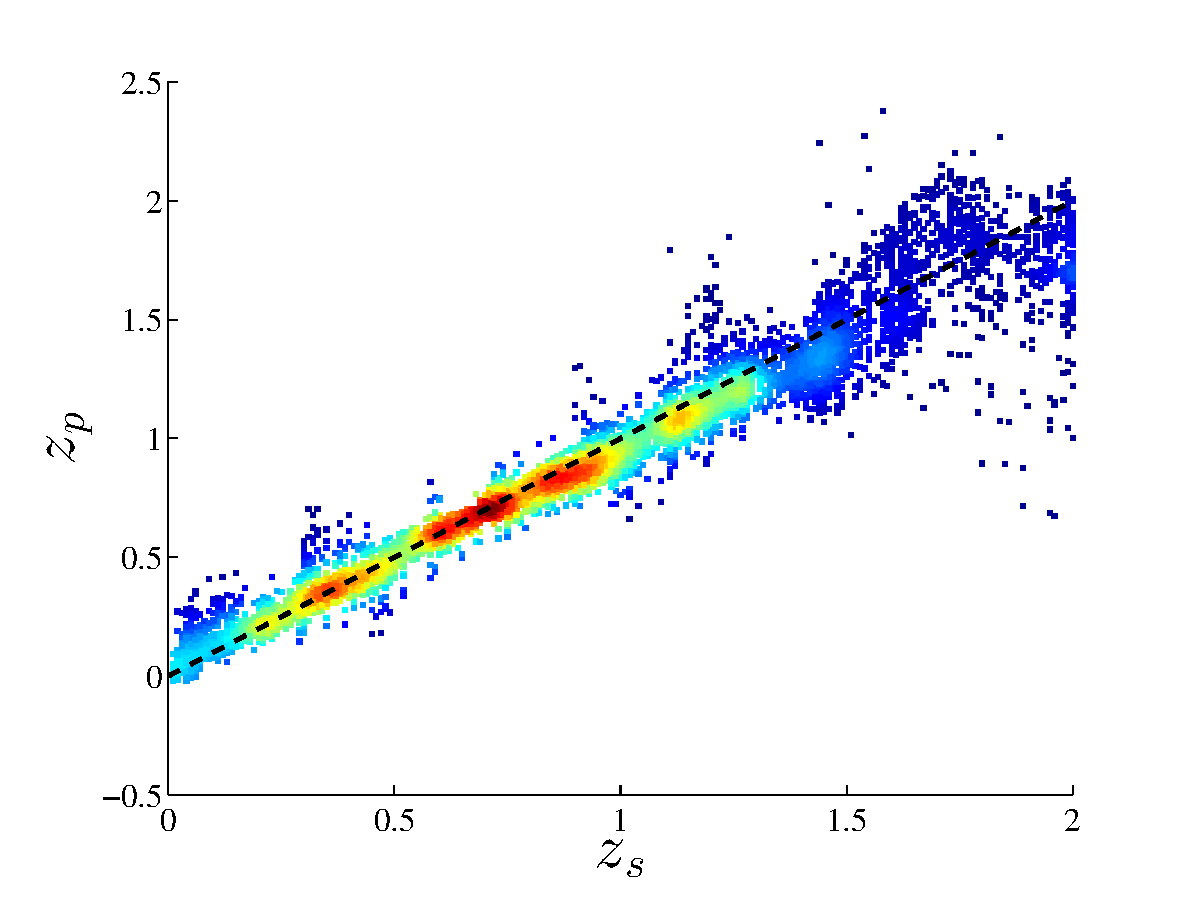
\includegraphics[width=\textwidth]{figures/22_J.eps}
                \caption{Joint}
        \end{subfigure}
        
        \caption{Density scatter plots of the true $z_{spec}$ vs the predicted $z_{phot}$ after training the GP-VC model with samples with $RIZ<23$ (top) and $RIZ<22$ (bottom) using $m=10$ basis functions with (a) zero mean, (b) linear regression and (c) joint linear and non-linear optimisation}
        \label{fig-RIZ-splits}
\end{figure*}


\subsection{Weighted Samples}
In this experiment, a comparison between the cost sensitive learning and the normal sum of squares for the GP-VC model is presented. Two different weight configurations are tested, the first is to assign an error cost to each sample equals to $1/\left(1+z_{spec}\right)^{2}$ to directly target the Euclid mission requirement (Normalised), and the second experiment is to weigh each sample according to the frequency of their true redshift to ensure balanced learning (Balanced).  Two additional measures are reported, the maximum $\Delta z$ and the maximum $\Delta z_{norm}$. The samples were grouped into bins of uniformly spaced intervals of 0.1, the box plots are shown in Figure \ref{fig-normal} for the normal weighting scheme and Figure \ref{fig-balanced} shows the results of the balanced training. The results from the figures show that the cost sensitive learning is more consistent across the redshift range as opposed to the normal sum of squares, especially in the high redshift regions were there is less data the confidence intervals are considerably smaller. The performance comparison for the normal, balanced and normalised training are summarised in Table \ref{table-normal-balanced}. Balanced training showed a better generalisation performance, as it outperformed the normal sum of squares objective on the test set and has lower maximum errors.

\begin{figure}
        \centering
        \begin{subfigure}[b]{\columnwidth}
                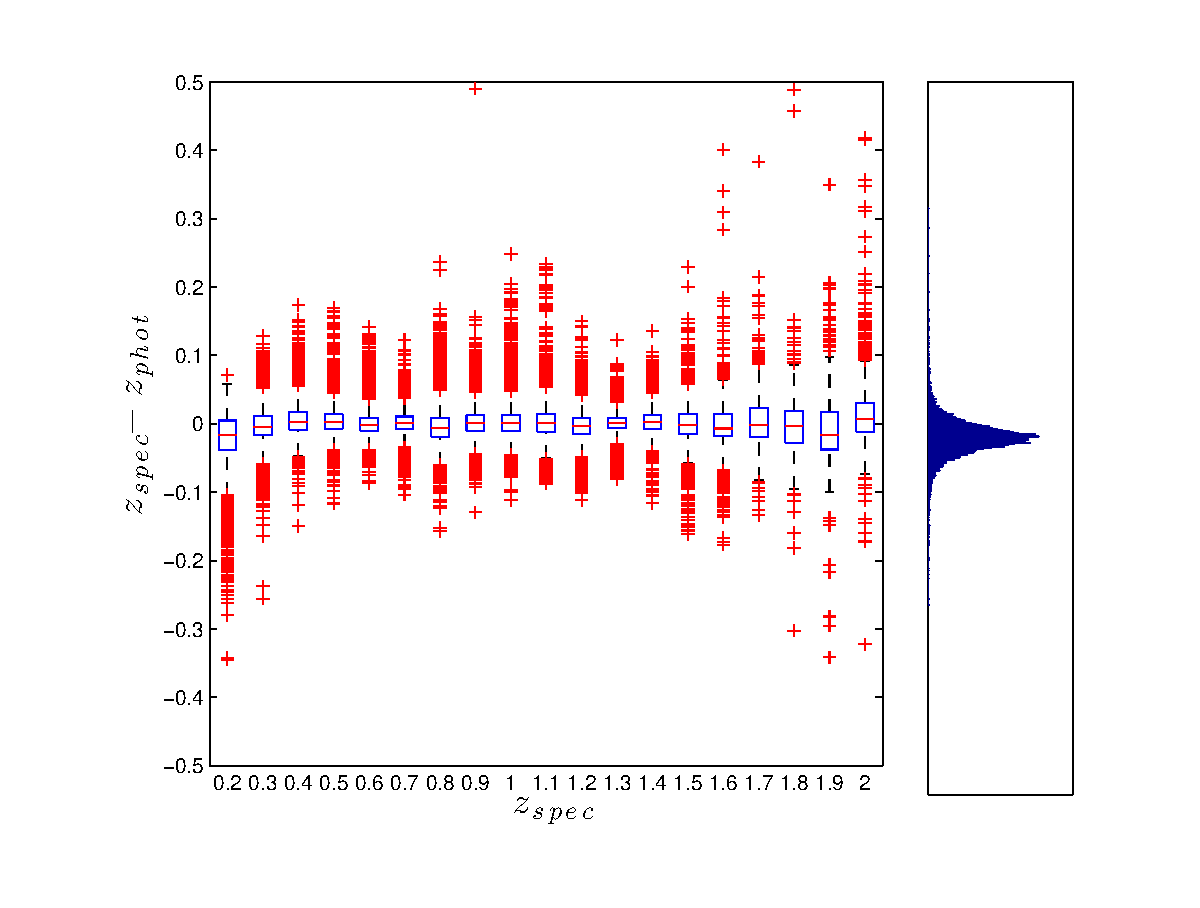
\includegraphics[width=\textwidth]{figures/Zspec-Zphot_normal.eps}
                \caption{Normal}
                \label{fig-normal}
        \end{subfigure}	
        \begin{subfigure}[b]{\columnwidth}
                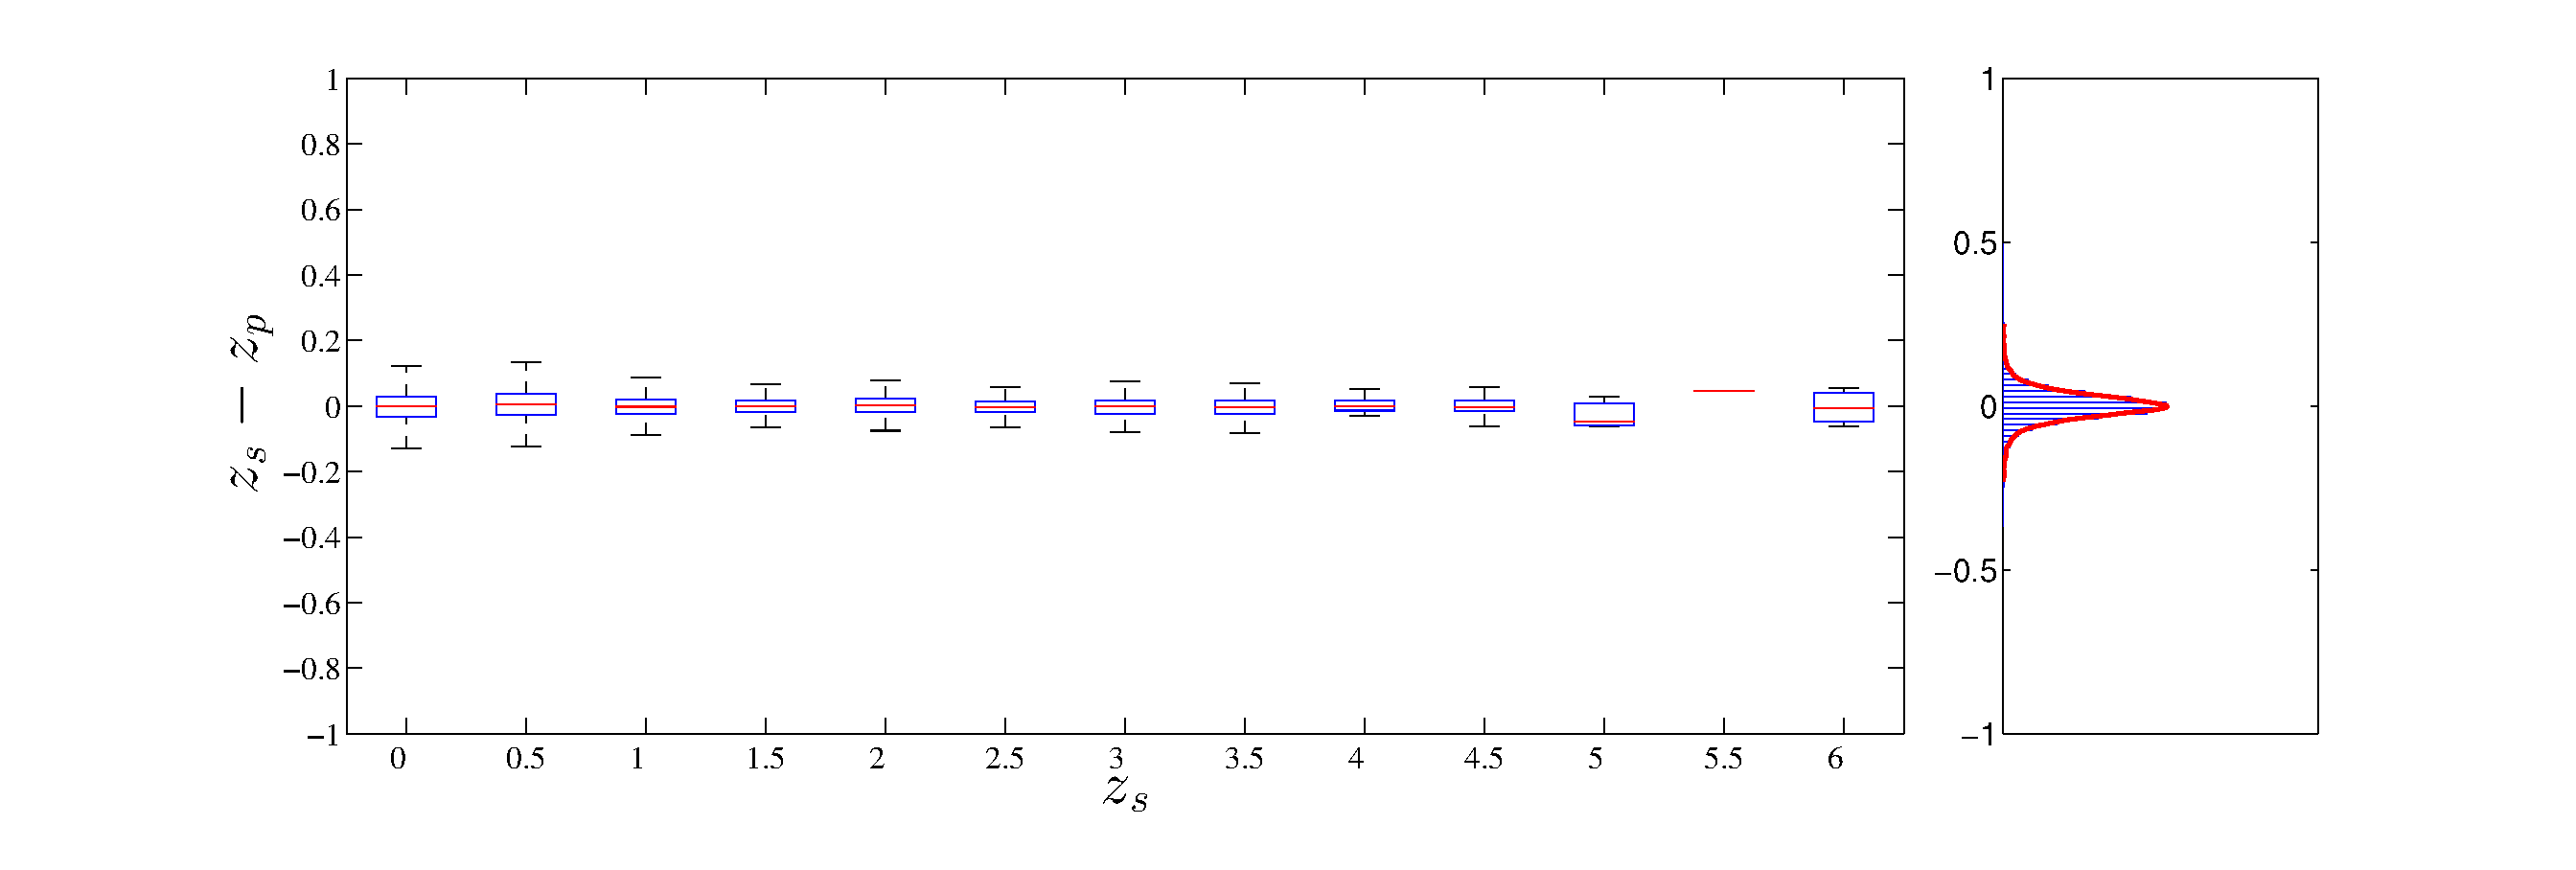
\includegraphics[width=\textwidth]{figures/Zspec-Zphot_balanced.eps}
                \caption{Balanced}
                \label{fig-balanced}
        \end{subfigure}
       \caption{Box plots of residual errors on the hold-out test set, showing median (bar), inter-quartile range (box) and range (whiskers) for (a) the direct sum of squared errors and (b) the balanced cost sensitive learning for the GV-VC model. All training was with $m=10$ basis functions for comparison. The right-most histograms are the empirical densities of errors.}
	\label{fig-normal-balanced}
\end{figure}

 \begin{table}
\caption{Performance measures of training the GP-VC model using $m=10$ basis functions and different weighting schemes.}
\begin{center}
  \begin{tabular}{| l | c | c | c | c |}
     				&	$\Delta z$	&	$max\left(\Delta z\right)$		&	$\Delta z_{norm}$		&	$max\left(\Delta z_{norm}\right)$	\\	\hline
	Normal		&	0.0247		&	0.3227			&	0.0148				&	0.2096				\\
	Balanced		&	\textbf{0.0213}	&	\textbf{0.2816}		&	0.0138				&	\textbf{0.1591}			\\
	Normalised	&	0.0237		&	0.4082			&	\textbf{0.0127}			&	0.1953				\\	\hline
  \end{tabular}
\end{center}
\label{table-normal-balanced}
\end{table}

\subsection{Size of the basis set}
In this test, all the models are cross compared by varying the number of basis functions $m$ from 5 to 200 by an increment of 5 to study the relationship between accuracy, complexity and speed. The plot of the $\Delta z$ as a function of $m$ is shown in Figure \ref{fig-rmses}, the $y$-axis is shown on a log scale for the purpose of visualisation. The stable GP showed the worst performance across the board, especially when the number of basis was low, while GP-VC on the other hand consistently outperformed the rest and most significantly when trained with a few number of basis. ANN outperformed GP-GL and GP-VL, but it did not scale well with complexity as it converged around $m=100$. All the models were trained using a sum of squares objective with no cost sensitive learning or prior mean function in this experiment. GP-VC satisfied the Euclid Mission's requirement was only $m=5$ basis, and when using $m=200$ was able to guarantee  a maximum normalised error less then the required for the mission. The  time complexities for each algorithm are shown in Table \ref{table-time-complexity} and the clock time in seconds, for a single iteration, are shown for various number of basis functions are shown in Figure \ref{fig-time-seconds}. The time experiment was conducted on a machine with a 3.0 GHz Intel Core i7 processor using Matlab 2014a. \footnote{Note that even though stableGP has a lower theoretical time complexity compared to GP-VC, it is significantly slower. This has to do with the particular choice of implementation and the development environment. The partial Cholesky decomposition implementation in stableGP \citep{stableGP} uses repeated loops which tends to perform poorly as it cannot exploit parallelised operations. The other methods on the other hand are based on matrix operations which utilise all the cores of the CPU by parallelising the operations.} We see from Figure \ref{fig-rmses} that all algorithms converged around $m=50$ with very little return in accuracy for the time spent beyond this point.

We note that although the \emph{training} complexity costs require effort for large numbers of basis functions, once all parameters are inferred we enjoy effectively a linear basis model performance running over unseen (test) data. We therefore consider the performance for a realistic, yet large, number of functions. 

 \begin{table}
\caption{The time complexity of each approach.}
\begin{center}
  \begin{tabular}{| l | l |}
     	Method		&	Time Complexity					\\	\hline
	ANN			&	$O\left(nmd\right)$					\\
	stable GP		&	$O\left(nm^{2}\right)$				\\
	GP-GL		&	$O\left(nm^{2}+nmd\right)$		\\	
	GP-VL		&	$O\left(nm^{2}+nmd\right)$		\\	
	GP-VC		&	$O\left(nm^{2}+nmd^{2}\right)$	\\	\hline
  \end{tabular}
\end{center}
\label{table-time-complexity}
\end{table}

\begin{figure}
        \centering
        
        \begin{subfigure}[b]{0.45\textwidth}
                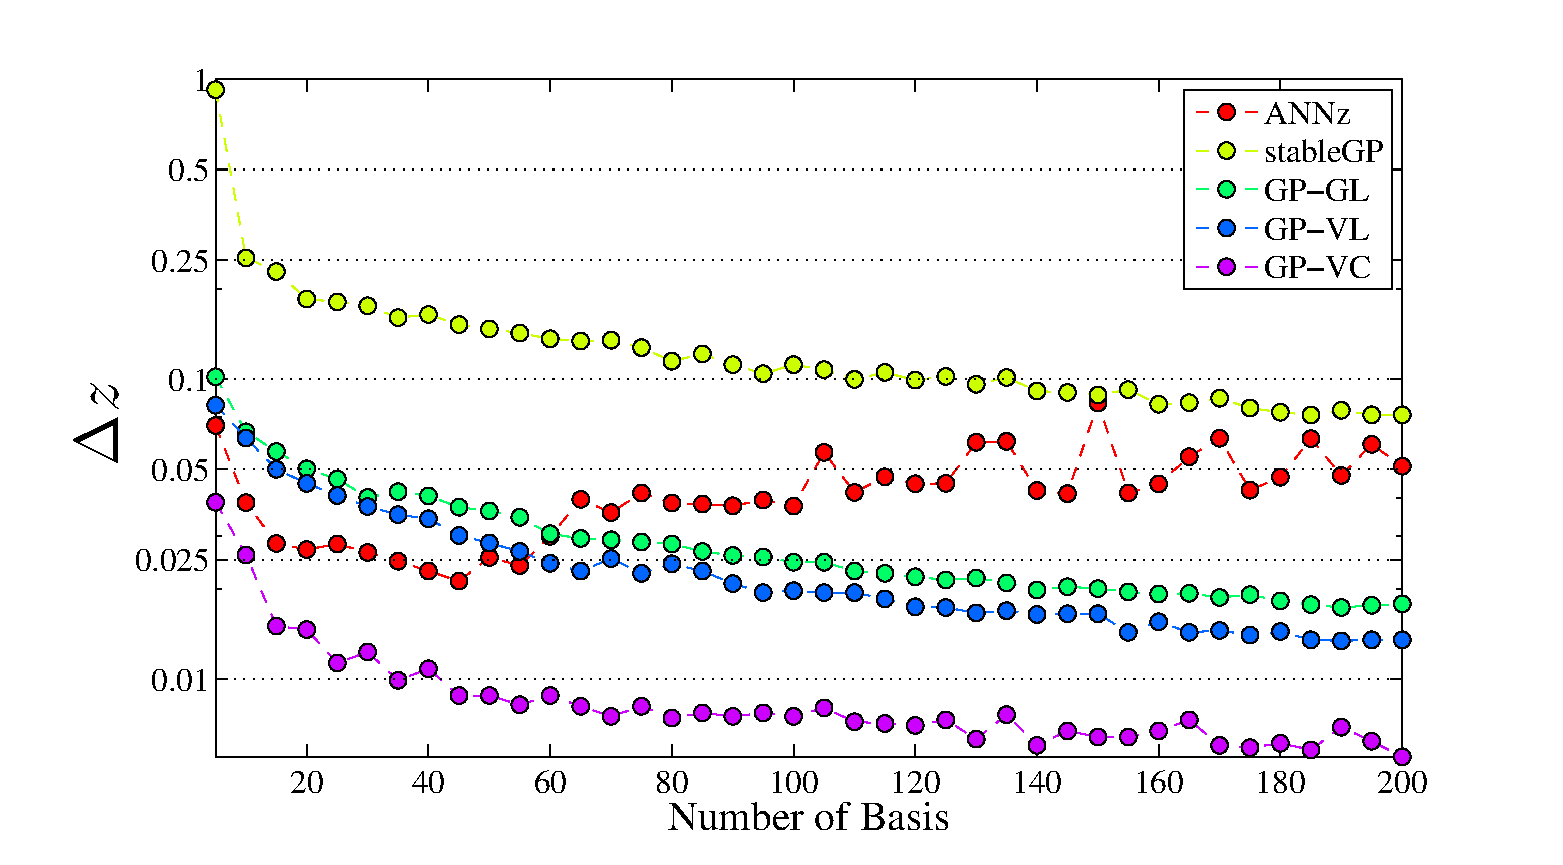
\includegraphics[width=\textwidth]{figures/different-basis.eps}
                 \caption{Root Mean Squared Error.}
                 \label{fig-rmses}
        \end{subfigure}
	 ~
       \begin{subfigure}[b]{0.45\textwidth}
                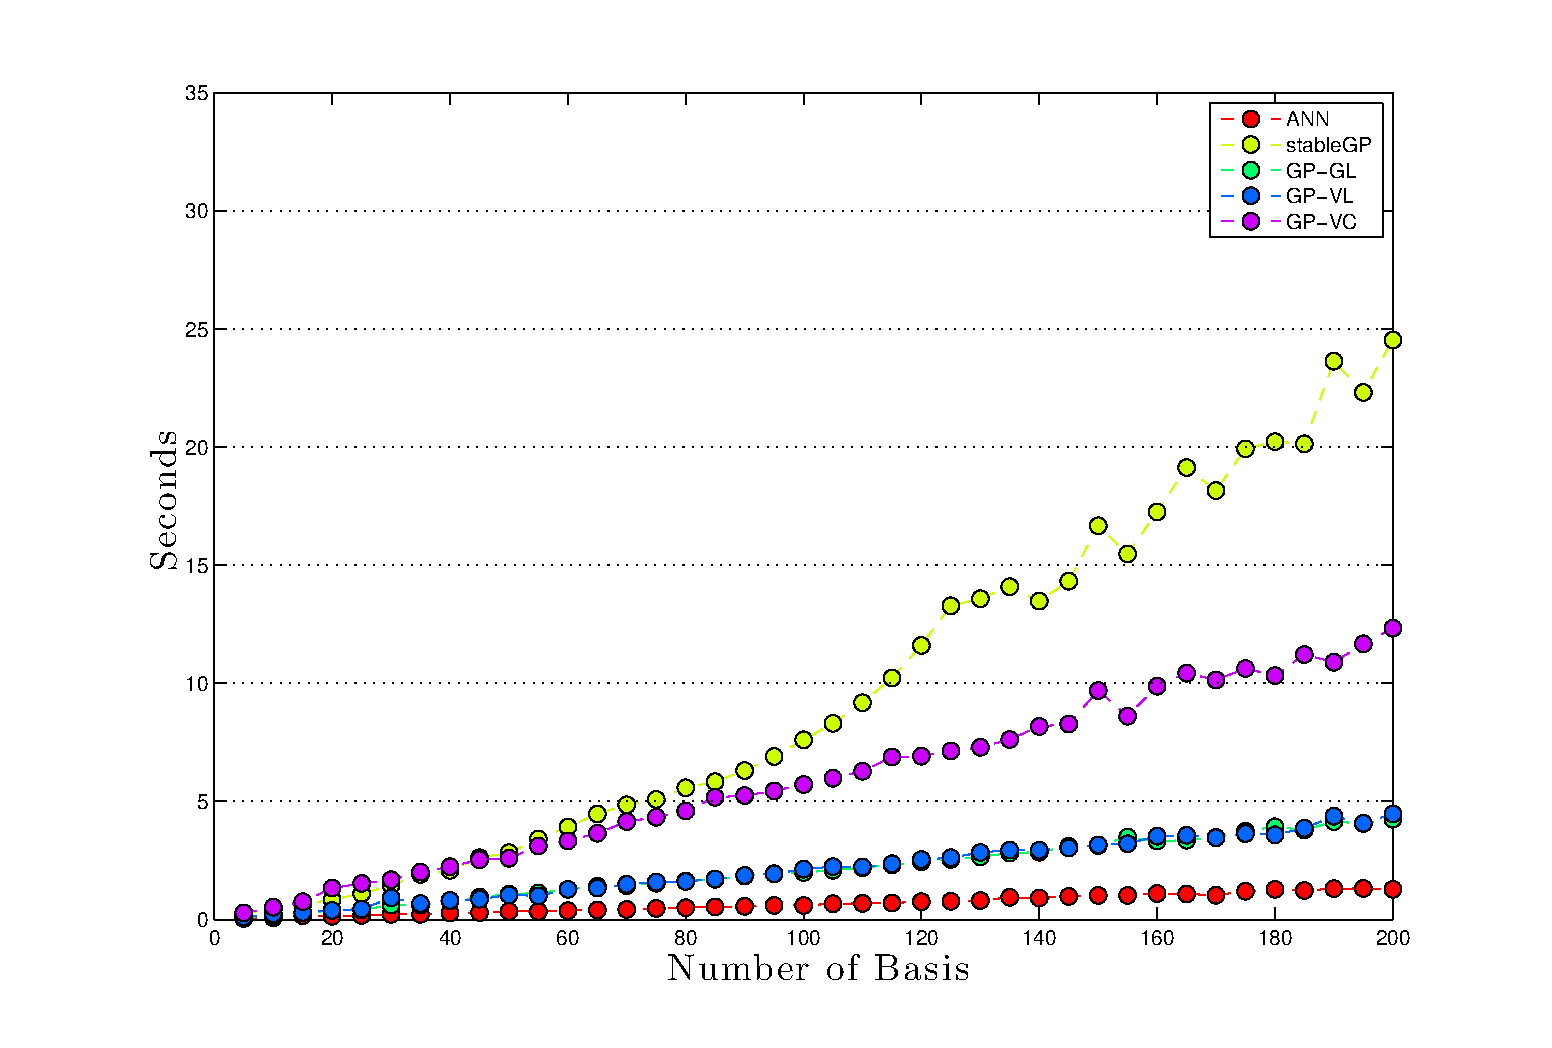
\includegraphics[width=\textwidth]{figures/times.eps}
                 \caption{Time.}
                 \label{fig-time-seconds}
        \end{subfigure}

       \caption{The root mean squares (a) and the time in seconds per iteration (b) as a function of $m$ for all the models.}	
\end{figure}

\subsection{Size of the training set}

In this experiment the generalisation performance of the GP-VC is tested by limiting the training set size to different percentage of the dataset. Given the expense of measuring redshifts spectroscopically, there is a strong incentive to reach the desired performance criteria with as small a training set as possible, although there will be some freedom to selectively target those sources which will best serve this training. The validation and test sets were set fixed to the same sets used in previous experiments to ensure consistent reporting on the same test set. The model was trained using various percentages from 5\% to 80\% and the $\Delta z$ as well as the $\Delta z_{norm}$ are reported for each percentage split in the plot shown in Figure \ref{fig-training-percentage}. The models were trained using the ``Joint'' prior optimisation, cost-sensitive learning and normalised weights using $m=200$ basis functions. The results from Figure \ref{fig-training-percentage} shows a stable generalisation performance for the GP-VC model with cost-sensitive learning even when using a limited training set size. The final GP-VC model to target the Euclid Space Mission was trained with $m=200$ basis functions normalised, balanced and with a joint mean optimisation reached a mean $\Delta z_{norm}=0.003$ and a $max\left(\Delta z_{norm}\right)=0.0468$ on the test set. The density scatter plot for the final model is shown in Figure \ref{fig-final-model}.

\begin{figure}
       \centering
        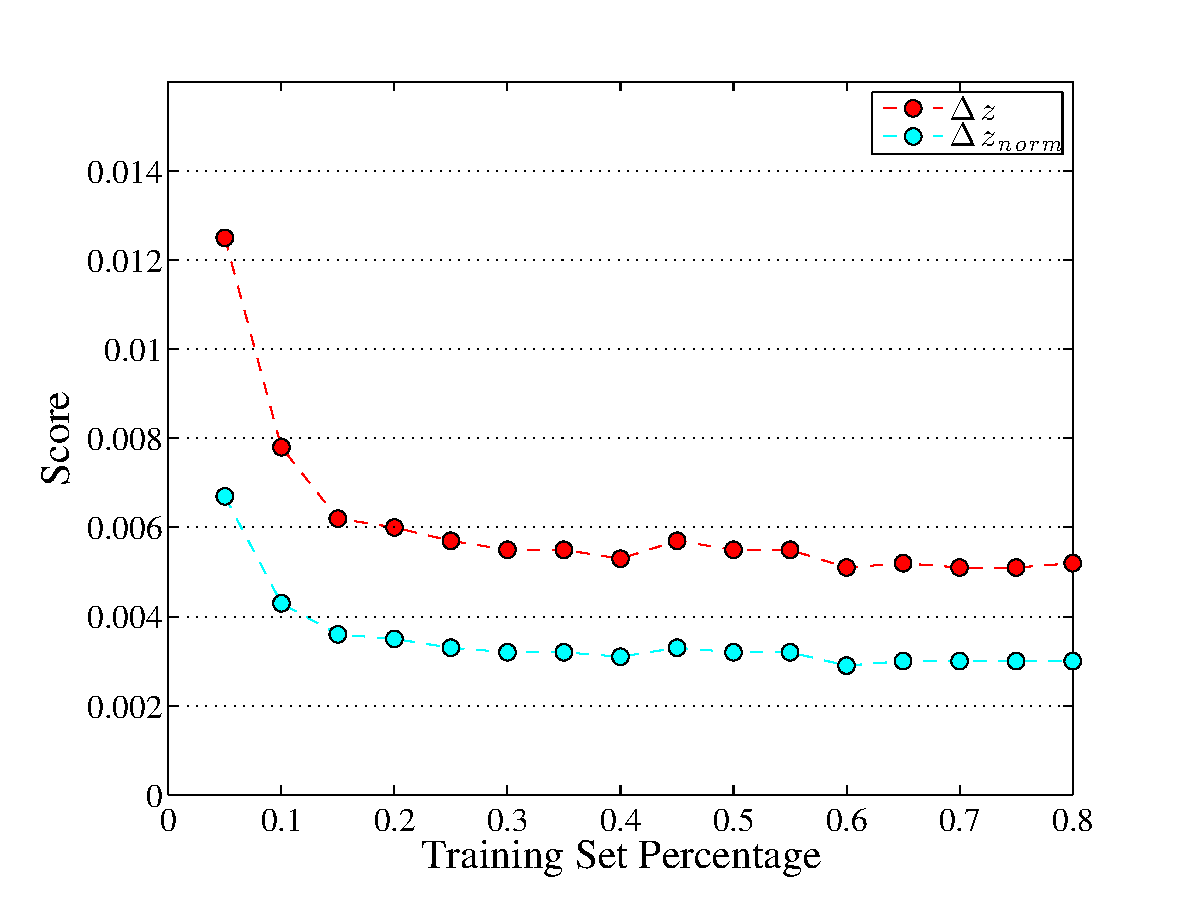
\includegraphics[width=\columnwidth]{figures/percentage.eps}
        \caption{The $\Delta z$ and $\Delta z_{norm}$ after training GP-VC models with $m=200$ basis functions with various training set percentage splits. }
       \label{fig-training-percentage}
\end{figure}

\begin{figure}
       \centering
        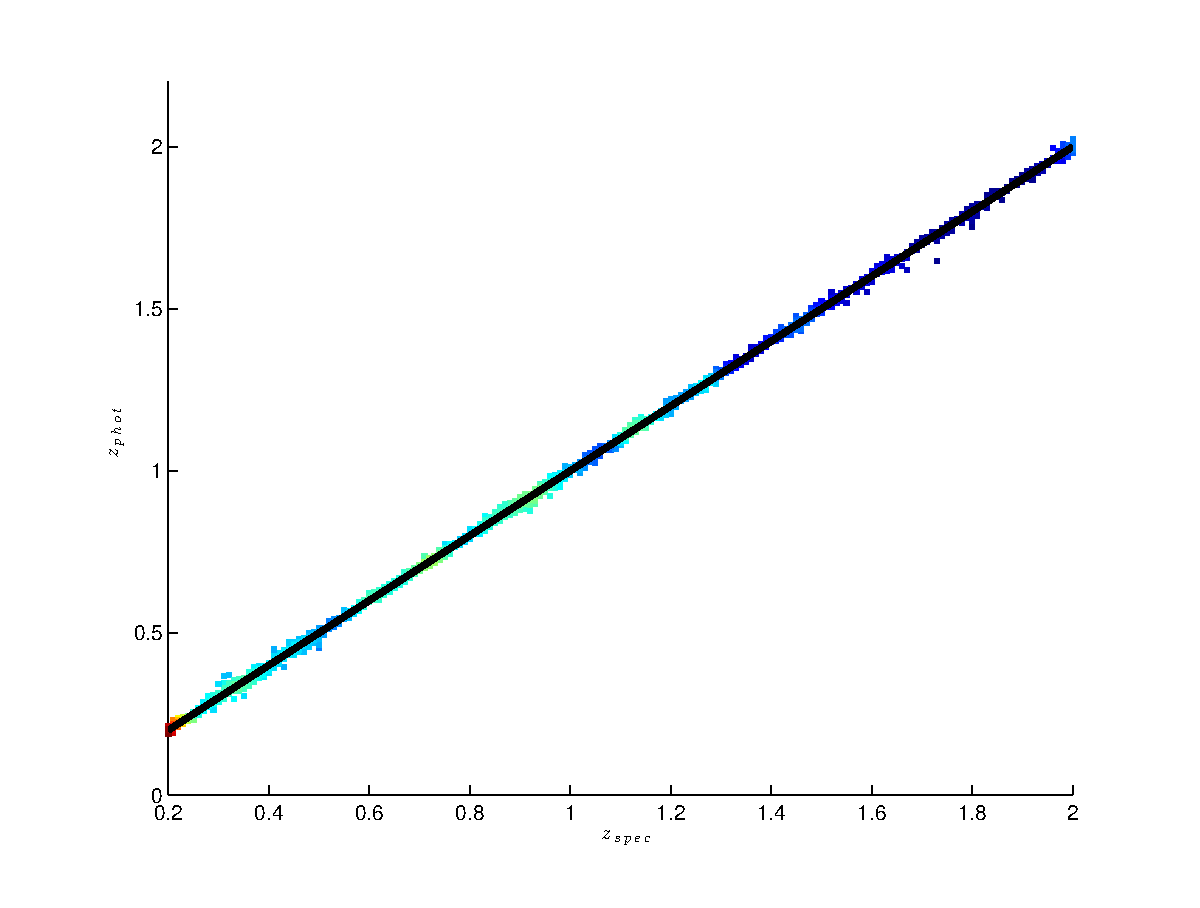
\includegraphics[width=\columnwidth]{figures/final-model.eps}
        \caption{The density scatter plot for the final GP-VC model trained using $m=200$ basis functions with a jointly optimised linear mean function, a balanced and normalised weights. }
       \label{fig-final-model}
\end{figure}

\section{Conclusion}
\label{sec-conclusion}
\textbf{SR: needs extra work here}

In this paper a sparse Gaussian process framework is presented and applied to photometric redshift estimation. The framework was able to out perform Artificial Neural Networks and sparse Gaussian processes with a global set of hyper-parameters. The performance increase is attributed to the handling of distribution bias via a weighting scheme integrated as part of the optimisation objective, parameterising each basis function with different covariances, and integrating the learning of the prior mean function to enhance the extrapolation performance of the model. The methods were applied to a simulated data set and the proposed approach consistently outperformed the other models on all measures while maintaining a low ration of model complexity to accuracy as scored by the Bayesian Information Criterion.


\footnotesize{
\bibliographystyle{mn2e}
\bibliography{sources}
}

\label{lastpage}
\end{document}
